%&pdflatex
\documentclass[pdftex,preprint,3p,times,numbers]{elsarticle}

\journal{Computer Physics Communications}

%\usepackage{moreverb}

\usepackage{hyperref}
\hypersetup{pdfborder={0 0 0}}

\usepackage{float}
\usepackage{wrapfig}
\usepackage{caption}
\usepackage{subcaption}
\usepackage{multirow}
\graphicspath{{images/}}

\usepackage[pdftex,usenames]{xcolor}

\usepackage{booktabs}
%\usepackage{colortbl}
\usepackage{multirow}

\usepackage{amsmath}
\usepackage{amssymb}
\usepackage[utf8x]{inputenc}
\usepackage[T1]{fontenc}

\usepackage{xspace}

\usepackage{xcolor}
\definecolor{Maroon}{cmyk}{0,0.87,0.68,0.32}
\definecolor{RoyalBlue}{cmyk}{1,0.50,0,0}
\definecolor{gray}{cmyk}{0.01,0.01,0.01,0.01}
\usepackage{listings}
\lstdefinelanguage{MyFortran}[95]{Fortran}{morecomment=[l]{\#},morestring=[d]',morekeywords={procedure,pass,deferred,non_overridable,generic,class,is}}
\lstdefinestyle{code}{%
  basicstyle=\footnotesize,%
  backgroundcolor=\color{gray},%
  language=MyFortran,%
  captionpos=b,%
  columns=fixed,%
  xleftmargin=10pt,%
  numbers=none,%
  numberstyle={\tiny},%
  keywordstyle=\color{RoyalBlue},%
  stringstyle={\sffamily},%
  texcl=true,%
  upquote=true,%
  commentstyle=\color{Maroon}%
}

\DeclareSymbolFont{extraup}{U}{zavm}{m}{n}
\DeclareMathSymbol{\vardiamond}{\mathalpha}{extraup}{87}
\definecolor{OMP}{RGB}{255,127,0}
\definecolor{MPI}{RGB}{0,127,255}
\definecolor{HYB}{RGB}{127,0,255}

\DeclareGraphicsExtensions{.pdf,.png,.jpg,.bmp,.mps}
\newcommand{\citeh}[1]{\citeauthor{#1} \citenum{#1}}

\renewcommand{\thesubfigure}{\Alph{subfigure}}

\begin{document}

\begin{frontmatter}

\title{FOODiE, Fortran Object oriented Ordinary Differential Equations integration library based on Abstract Calculus Pattern}

\author[insean]{Zaghi S.\corref{cor1}\fnref{sz}}
\ead{stefano.zaghi@cnr.it}
\fntext[sz]{Ph. D., Aerospace Engineer, Research Scientist, Dept. of Computational Hydrodynamics at CNR-INSEAN.}
\address[insean]{CNR-INSEAN, Istituto Nazionale per Studi ed Esperienze di Architettura Navale, Via di Vallerano 139, Rome, Italy, 00128}
\cortext[cor1]{Corresponding author}

\author[rsmas]{Curcic M.\fnref{mc}}
\ead{milan@orca.rsmas.miami.edu}
\fntext[mc]{Ph.D. Meteorology and Physical Oceanography, Research Scientist, Dept. of Ocean Sciences Rosenstiel School of Marine and Atmospheric Science at University of Miami}
\address[rsmas]{Ocean Sciences Rosenstiel School of Marine and Atmospheric Science, University of Miami, 4600 Rickenbacker Causeway Miami, FL 33149-1098 +1 305.421.4000}

\author[sourcery]{Rouson D.\fnref{dr}}
\ead{damian@sourceryinstitute.org}
\fntext[dr]{Ph.D. Mechanical Engineering, Founder and President Sourcery Institute and Sourcery, Inc.}
\address[sourcery]{Sourcery Institute 482 Michigan Ave., Berkeley, CA 94707}

\author[sourcery]{Beekman I.\fnref{iz}}
\ead{izaak@izaakbeekman.com}
\fntext[iz]{Graduate Research Assistant, Princeton/UMD CCROCCO LAB}

\begin{abstract}
To be written.
\end{abstract}

\begin{keyword}
  Ordinary Differential Equations (ODE) \sep
  Partial Differential Equations (PDE) \sep
  Object Oriented Programming (OOP) \sep
  Abstract Calculus Pattern (ACP) \sep
  Fortran \sep
\end{keyword}

\end{frontmatter}

{\bf PROGRAM SUMMARY}

\begin{small}
\noindent
\emph{Manuscript Title:} FOODiE, Fortran Object oriented Ordinary Differential Equations integration library based on Abstract Calculus Pattern \\
\emph{Authors:} Zaghi, S., Curcic, M., Rouson, D., Beekman, I. \\
\emph{Program title:} FOODiE \\
\emph{Journal Reference:} \\
\emph{Catalogue identifier:} \\
\emph{Licensing provisions:} GNU General Public License (GPL) v3 \\
\emph{Programming language:} Fortran (standard 2008 or newer); developed and tested with GNU gfortran 5.2 or newer \\
\emph{Computer(s) for which the program has been designed:} designed for shared-memory multi-cores workstations and for hybrid distributed/shared-memory supercomputers, but any computer system with a Fortran (2008+) compiler is suited \\
\emph{Operating system(s) for which the program has been designed:} designed for POSIX architecture and tested on GNU/Linux one \\
\emph{RAM required to execute with typical data: bytes:} $[1MB,1GB]\times core$, simulation-dependent \\
\emph{Has the code been vectorised or parallelized?:} the library is not aware of the parallel back-end, it providing a high-level models, but the provided tests suite shows parallel usage by means of MPI library and OpenMP paradigm \\
\emph{Number of processors used:} tested up to 256 \\
\emph{Supplementary material:}    \\
\emph{Keywords:} ODE, PDE, OOP, ACP, Fortran \\
\emph{CPC Library Classification:} 4.3 Differential Equations, 4.10 Interpolation, 12 Gases and Fluids \\
\emph{External routines/libraries used:} \\
\emph{CPC Program Library subprograms used:} \\
\emph{Nature of problem:} \\
Numerical integration of (general) Ordinary Differential Equations system \\
\emph{Solution method:} \\
\emph{Restrictions:} \\
\emph{Unusual features:} \\
\emph{Additional comments:} \\
\emph{Running time:} \\
\emph{References:} \\
% \begin{thebibliography}{0}
% \end{thebibliography}
\end{small}

\section{Introduction}\label{sec:introduction}
\subsection{Background}

Initial Value Problem (IVP, or Cauchy problem) constitutes a class of mathematical models of paramount relevance, it being applied to the modelling of a wide range of problems. Briefly, an IVP is an Ordinary Differential Equations system (ODE) coupled with specified initial values of the unknown state variables, the solution of which are searched at a given time after the initial time considered.

The prototype of IVP can be expressed as:
\begin{equation}
  \begin{matrix}
  U_t = R(t,U) \\
  U_0 = U(t_0)
  \end{matrix}
\label{eq:IVP}
\end{equation}
where $U(t)$ is the vector of state variables being a function of the time-like independent variable $t$, $U_t = \frac{dU}{dt} = R(t,U)$ is the (vectorial) residuals function and $U(t_0)$ is the (vectorial) initial conditions, namely the state variables function evaluated at the initial time $t_0$. In general, the residuals function $R$ is a function of the state variable $U$ through which it is a function of time, but it can be also a direct function of time, thus in general $R=R(t,U(t))$ holds.

The problem prototype \ref{eq:IVP} is ubiquitous in the mathematical modelling of physical problems: essentially whenever an \emph{evolutionary} phenomenon is considered the prevision (simulation) of the future solutions involves the solution of an IVP. As a matter of facts, many physical problems (fluid dynamics, chemistry, biology, evolutionary-anthropology, etc...) are described by means of an IVP.

It is worth noting that the state vector variables $U$ and its corresponding residuals function $U_t = \frac{dU}{dt} = R(t,U)$ are \emph{problem dependent}: the number and the meaning of the state variables as well as the equations governing their evolution (that are embedded into the residuals function) are different for the Navier-Stokes conservation laws with respect the Burgers one, as an example. Nevertheless, the \emph{solvers} used for the prediction of the Navier-Stokes equations evolution (hereafter the \emph{solution}) are the same that are used for Burgers equations time-integration. As a consequence, the solution of the IVP model prototype can be generalized, allowing the application of the same solver to many different problems, thus eliminating the necessity to re-implement the same solver for each different problem.

FOODiE library is designed for solving the generalized IVP \ref{eq:IVP}, it being completely unaware of the actual problem's definition. FOODiE library provides a high-level, well-documented, simple Application Program Interface (API) for many well-known ODE integration solvers, its aims being twofold:

\begin{itemize}
  \item provide a robust set of ODE solvers ready to be applied to a wide range of different problems;
  \item provide a simple framework for the rapid development of new ODE solvers.
\end{itemize}

{\color{red} Add citations to IVP, Cauchy, ODE references.}

\subsection{Related Works}

{\color{red} To be written.}

\subsection{Motivations and Aims}

FOODiE library must:

\begin{itemize}
  \item be written in modern Fortran (standard 2008 or newer);
  \item be written by means of Object Oriented Programming (OOP) paradigm;
  \item be well documented;
  \item be Tests Driven Developed (TDD);
  \item be collaboratively developed;
  \item be free.
\end{itemize}

FOODiE, meaning Fortran Object oriented Ordinary Differential Equations integration library, has been developed with the aim to satisfy the above specifications. The present paper is its first comprehensive presentation.

The Fortran (Formula Translator) programming language is the \emph{de facto} standard into computer science field: it strongly facilitates the effective and efficient translation of (even complex) mathematical and numerical models into an operative software without compromise on computations speed and accuracy. Moreover, its simple syntax is suitable for scientific researchers that are interested (and skilled) in the physical aspects of the numerical computations rather than computer technicians. Consequently, we develop FOODiE using Fortran language: FOODiE is written by research scientists for research scientists.

One key-point of the FOODiE development is the \emph{problem generalization}: the problem solved must be the IVP \ref{eq:IVP} rather than any of its actual definitions. Consequently, we must rely on a \emph{generic} implementation of the solvers. To this aim, OOP is very useful: it allows to express IVP \ref{eq:IVP} in a very concise and clear formulation that is really generic. In particular, our implementation is based on \emph{Abstract Calculus Pattern} (ACP) concept.

\paragraph{The Abstract Calculus Pattern}
The abstract calculus pattern provides a simple solution for the connection between the very high-level expression of IVP \ref{eq:IVP} and the eventual concrete (low-level) implementation of the ODE problem being solved. ACP essentially constitutes a \emph{contract} based on an Abstract Data Type (ADT): we specify an ADT supporting a certain set of mathematical operators (differential and integral ones) and implement FOODiE solvers only on the basis of this ADT. FOODiE clients must formulate the ODE problem under integration defining their own concrete extensions of our ADT (implementing all the deferred operators). Such an approach defines the abstract calculus pattern: FOODiE solvers are aware of only the ADT, while FOODiE clients extend the ADT for defining the concrete ODE problem.

Is is worth noting that this ACP emancipates the solvers implementations from any low-level problem-dependent details: the ODE solvers developed with this pattern are extremely concise, clear, maintainable and less errors-prone with respect a low-level (non abstract) pattern. Moreover, the FOODiE clients can use solvers being extremely robust: as a matter of facts, FOODiE solvers are expressed in a formulation very close to the mathematical one and are tested on an extremely varying family of problems. As shown in the following, such a great flexibility does not compromise the computational efficiency.

The present paper is organized as following: in section \ref{sec:MNmodels} a brief description of the mathematical and numerical methods currently implemented into FOODiE is presented; in section \ref{sec:API} a detailed discussion on the implementation specifications is provided by means of an analytical code-listings review; in section \ref{sec:Tests} a verification analysis on the results of FOODiE applications is presented; section \ref{sec:parallel} provides an analysis of FOODiE performances under parallel frameworks scenario like the OpenMP and MPI paradigms; finally, in section \ref{sec:conclusions} concluding remarks and perspectives are depicted.

{\color{red} Add citations to Fortran standards, OOP, TDD, free software, ACP, ADT, Rouson's book references.}

\section{Mathematical and Numerical Models}\label{sec:MNmodels}

In many (most) circumstances, the solution of equation \ref{eq:IVP} cannot be computed in a closed, exact form (even if it exists and is unique) due to the complexity and nature of the residuals functions, that is often non linear. Consequently, the problem is often solved relying on a numerical approach: the solution of system \ref{eq:IVP} at a time $t^n$, namely $U(t^n)$, is approximated by a subsequent time-marching approximations $U_0=u_0 \rightarrow u_1 \rightarrow u_2 \rightarrow ... \rightarrow u_N\approx U(t^n)$ where the relation $u_i \rightarrow u_{i+1}$ implies a \emph{stepping, numerical integration} from the time $t^i$ to time $t^{i+1}$ and $N$ is the total number of numerical time steps necessary to evolve the initial conditions toward the searched solution $U(t^n)$. To this aim, many numerical schemes have been devised. Notably, the numerical schemes of practical usefulness must posses some necessary proprieties such as \emph{consistency} and \emph{stability} to ensure that the numerical approximation \emph{converges} to the exact solution as the numerical time step tends to zero. A detailed discussion of these details is out the scope of the present work and is omitted. Here, we briefly recall some classifications necessary to introduce the schemes implemented into the FOODiE library.

A non comprehensive classification of the most widely used schemes could distinguish between \emph{multi-step} versus \emph{one-step} schemes and between \emph{explicit} versus \emph{implicit} schemes.

Essentially, the multi-step schemes have been developed to obtain an accurate approximation of the subsequent numerical steps using the informations contained into the previously computed steps, thus this approach relates the next step approximation to a set of the previously computed steps. On the contrary, a one-step scheme evolves the solution toward the next step using only the information coming from the current time approximation. In the framework of one-step schemes family an equivalent accurate approximation can be obtained by means of a multi-stage approach as the one due to Runge-Kutta. The current version of FOODiE provides schemes belonging to both these families.

The other ODE solvers classification concerns with explicit or implicit nature of the schemes employed. Briefly, an explicit scheme computes the next step approximation using the previously computed steps at most to the current time, whereas an implicit scheme uses also the next step approximation (that is the unknown), thus it requires extra computations. The implicit approach is of practical use for \emph{stiff} systems where the usage of explicit schemes could require an extremely small time step to evolve in a \emph{stable} way the solution. Currently, FOODiE provides only explicit solvers.

FOODiE currently implements the following ODE schemes:

\begin{itemize}
  \item one-step schemes:
    \begin{itemize}
      \item explicit forward Euler scheme, it being $1^{st}$ order accurate;
      \item explicit Runge-Kutta schemes:
        \begin{itemize}
          \item TVD/SSP Runge-Kutta schemes:
            \begin{itemize}
              \item 2-stages, it being $2^{nd}$ order accurate;
              \item 3-stages, it being $3^{rd}$ order accurate;
              \item 5-stages, it being $4^{th}$ order accurate;
              \end{itemize}
          \item low storage Runge-Kutta schemes:
            \begin{itemize}
              \item 5-stages 2N registers schemes, it being $4^{th}$ order accurate;
              \end{itemize}
          \end{itemize}
      \end{itemize}
  \item multi-step schemes:
    \begin{itemize}
      \item Adams-Bashforth schemes:
        \begin{itemize}
          \item 2-steps, it being $2^{nd}$ order accurate;
          \item 3-steps, it being $3^{rd}$ order accurate;
          \item 4-steps, it being $4^{th}$ order accurate;
          \end{itemize}
        \item Leapfrog schemes\footnote{Leapfrog method is a 2-steps solver being, in general $2^{nd}$ order accurate, but mostly \emph{unstable}. It is well suited for periodic/oscillatory problems, thus the error is generally categorized accordingly to the phase and amplitude errors: the unfiltered scheme provides a $2^{nd}$ order error on phase approximation while the amplitude error is null. However, the unfiltered scheme is mostly unstable, thus many filters have been devised. In general, the filters retain the accuracy on the phase error, while affect the amplitude one.}:
        \begin{itemize}
          \item 2-steps unfiltered, it being $2^{nd}$ order accurate, but mostly \emph{unstable};
          \item 2-steps Robert-Asselin filtered, it being $1^{st}$ order accurate (on \emph{amplitude error});
          \item 2-steps Robert-Asselin-Williams filtered, it being $3^{rd}$ order accurate (on \emph{amplitude error});
          \end{itemize}
      \end{itemize}
  \end{itemize}

{\color{red} Add citations to all solvers reference papers.}

\subsection{The explicit forward Euler scheme}

The explicit forward Euler scheme for ODE integration is probably the simplest solver ever devised. Considering the system \ref{eq:IVP}, the solution (approximation) of the state vector $U$ at the time $t^{n+1}=t^n+\Delta t$ assuming to known the solution at time $t^n$ is:

\begin{equation}
  U\left(t^{n+1}\right) = U\left(t^n\right) +\Delta t \cdot R\left[t^n, U\left(t^n\right)\right]
\label{eq:solver-euler}
\end{equation}
where the solution at the new time step is computed by means of only the current time solution, thus this is an explicit scheme. The solution is an approximation of $1^{st}$ order, the local truncation error being $O(Dt^2)$. As well known, this scheme has an absolute (linear) stability locus equals to $|1+\Delta t \lambda|\le 1$ where $\lambda$ contains the eigenvalues of the linear (or linearized) Jacobian matrix of the system.

This scheme is Total Variation Diminishing (TVD), thus satisfies the maximum principle (or the equivalent positivity preserving property).

{\color{red} Add citations.}

\subsection{The explicit TVD/SSP Runge-Kutta class of schemes}

Runge-Kutta methods belong to the more general multi-stage family of schemes. This kind of schemes has been designed to achieve a more accurate solution than the $1^{st}$ Euler scheme, but without increasing the number of time steps used, as it is done with the multi-step schemes. Essentially, the high order of accuracy is obtained by means of \emph{intermediate values} (the stages) of the solution and its derivative are generated and used within a single time step. This commonly implies the allocation of some auxiliary memory registers for storing the intermediate stages.

Notably, the multi-stage schemes class has the attractive property to be \emph{self-starting}: the high order accurate solution can be obtained directly from the previous one, without the necessity to compute \emph{before} a certain number of previous steps, as it happens for the multi-step schemes. Moreover, one-step multi-stage methods are suitable for adaptively-varying time-step size (that is also possible for multi-step schemes, but at a cost of more complexity) and for discontinuous solutions, namely discontinued solutions happening at a certain time $t*$ (that in a multi-step framework can involve an overall accuracy degradation).

In general, the TVD/SSP Runge-Kutta schemes provided by FOODiE library are written by means of the following algorithm:
\begin{equation}
  U^{n+1} = U^{n} + \Delta t \cdot\sum\limits_{s=1}^{N_{s}}{\beta_s K_s}
\label{eq:RK}
\end{equation}
where $N_s$ is the number of Runge-Kutta stages used and $K_s$ is the $s^{th}$ stage defined as:
\begin{equation}
  K_s = R\left(t^n + \gamma_s \Delta t, U^n+\Delta t\sum\limits_{l=1}^{s-1}{\alpha_{s,l} K_l} \right)
\label{eq:RK-stage}
\end{equation}
It is worth noting that the equations \ref{eq:RK} and \ref{eq:RK-stage} contain also implicit schemes. A scheme belonging to this family is operative once the coefficients $\alpha,\, \beta,\, \gamma$ are provided. We represent these coefficients using the Butcher's table, that for an explicit scheme where $\gamma_1=\alpha_{1,*}=\alpha_{i,i}=0$ has the form reported in table \ref{tab:butcher-table}.

\begin{table}[!ht]
\caption{Butcher's table for explicit Runge-Kutta schemes}\label{tab:butcher-table}
\centering
\resizebox{0.40\textwidth}{!}{%
\begin{tabular}{c|ccccc}
 $\gamma_2$     & $\alpha_{2,1}$   &                  &          &                      &              \\
 $\gamma_3$     & $\alpha_{3,1}$   & $\alpha_{3,2}$   &          &                      &              \\
 $\vdots$       & $\vdots$         &                  & $\ddots$ &                      &              \\
 $\gamma_{N_s}$ & $\alpha_{N_s,1}$ & $\alpha_{N_s,2}$ & $\cdots$ & $\alpha_{N_s,N_s-1}$ &              \\
 \hline
                & $\beta_1$        & $\beta_2$        & $\cdots$ & $\beta_{N_s-1}$      & $\beta_{N_s}$\\
\end{tabular}}
\end{table}

The equations \ref{eq:RK} and \ref{eq:RK-stage} show that Runge-Kutta methods do not require any additional differentiations of the ODE system for achieving high order accuracy, rather they require additional evaluations of the residuals function $R$.

The nature of the scheme and the properties of the solutions obtained depend on the number of stages and on the value of the coefficients selected. Currently, FOODiE provides 3 Runge-Kutta schemes having TVD or Strong Stability Preserving (SSP) propriety (thus they being suitable for ODE systems involving rapidly changing non linear dynamics) the Butcher's coefficients of which are reported in tables \ref{tab:RK-TVD-butcher-2}, \ref{tab:RK-SSP-butcher-3}, \ref{tab:RK-SSP-butcher-5}.

\begin{table}[!ht]
  \centering
  \caption{Butcher's table of 2 stages, $2^{nd}$ order, Runge-Kutta TVD scheme\label{tab:RK-TVD-butcher-2}}
  \resizebox{0.15\textwidth}{!}{%
  \begin{tabular}{c|cc}
   1 & 1 & 0       \\
   \hline
       & 1/2 & 1/2   \\
  \end{tabular}}
\end{table}

\begin{table}[!ht]
  \centering
  \caption{Butcher's table of 3 stages, $3^{rd}$ order, Runge-Kutta SSP scheme\label{tab:RK-SSP-butcher-3}}
  \resizebox{0.20\textwidth}{!}{%
  \begin{tabular}{c|ccc}
   1   & 1   &     &      \\
   1/2 & 1/4 & 1/4 &      \\
   \hline
       & 1/6 & 1/6 & 2/3  \\
  \end{tabular}}
\end{table}

\begin{table}[!ht]
  \centering
  \caption{Butcher's table of 5 stages, $4^{th}$ order accurate, Runge-Kutta SSP scheme\label{tab:RK-SSP-butcher-5}}
  \resizebox{0.99\textwidth}{!}{%
  \begin{tabular}{c|ccccc}
   0.39175222700392 & 0.39175222700392 &                  &                  &                  &                  \\
   0.58607968896779 & 0.21766909633821 & 0.36841059262959 &                  &                  &                  \\
   0.47454236302687 & 0.08269208670950 & 0.13995850206999 & 0.25189177424738 &                  &                  \\
   0.93501063100924 & 0.06796628370320 & 0.11503469844438 & 0.20703489864929 & 0.54497475021237 &                  \\
   \hline
                    & 0.14681187618661 & 0.24848290924556 & 0.10425883036650 & 0.27443890091960 & 0.22600748319395 \\
  \end{tabular}}
\end{table}
The absolute stability locus depends on the coefficients selected, however, as a general principle, we can assume that greater is the stages number and wider is the stability locus on equal accuracy orders.

It is worth noting that FODDiE also provides a one-stage TVD Runge-Kutta solver that reverts back to the explicit forward Euler scheme: it can be used, for example, into a Recursive Order Reduction (ROR) framework that automatically checks some properties of the solution and, in case, reduces the order of the Runge-Kutta solver until those properties are obtained.

{\color{red} Add citations.}

\subsection{The explicit low storage Runge-Kutta class of schemes}

As aforementioned, standard Runge-Kutta schemes have the drawback to require $N_S$ auxiliary memory registers to store the necessary stages data. In order to make an efficient use of the available limited computer memory, the class of low storage Runge-Kutta scheme was devised. Essentially, the standard Runge-Kutta class (under some specific conditions) can be reformulated allowing a more efficient memory management. Currently FOODiE provides a class of \emph{2N registers} storage Runge-Kutta schemes, meaning that the storage of all stages requires only 2 registers of memory with a \emph{word} length $N$ (namely the length of the state vector) in contrast to the standard formulation where $N_s$ registers of the same length $N$ are required. This is a dramatic improvement of memory efficiency especially for schemes using a high number of stages ($N_s \ge 4$) where the memory necessary is an half with respect the original formulation. Unfortunately, not all standard Runge-Kutta schemes can be reformulated as a low storage one.

Following the Williamson's approach the standard coefficients are reformulated to the coefficients vectors $A$, $B$ and $C$ and the Runge-Kutta algorithm becomes:

\begin{equation}
\begin{matrix}
  K_1 = U\left(t^n\right) \\
  K_2 = 0 \\
  \left.\begin{matrix}
    K_2 = A_s K_2 + \Delta t \cdot R\left(t^n + C_s \Delta t, K_1\right) \\
    K_1 = K_1 + B_s K_2
  \end{matrix}\right\} s=1,2,...N_s\\
  U\left(t^{n+1}\right) = K_1
  \end{matrix}
\label{eq:RK-ls}
\end{equation}

Currently FOODiE provides only one 5 stages, $4^{th}$ order, 2N registers explicit scheme, the coefficients of which are listed in table \ref{tab:RK-ls-5}.

\begin{table}[!ht]
  \centering
  \caption{Williamson's table of 5 stages, $4^{th}$ order, Runge-Kutta low storage scheme\label{tab:RK-ls-5}}
  \resizebox{0.40\textwidth}{!}{%
  \begin{tabular}{ccc}
       $A$                                    & $B$                                    & $C$                                   \\
    \hline
       $ 0                                  $ & $\frac{1432997174477}{9575080441755 }$ & $ 0                                 $ \\
       $-\frac{567301805773 }{1357537059087}$ & $\frac{5161836677717}{13612068292357}$ & $\frac{1432997174477}{9575080441755}$ \\
       $-\frac{2404267990393}{2016746695238}$ & $\frac{1720146321549}{2090206949498 }$ & $\frac{2526269341429}{6820363962896}$ \\
       $-\frac{3550918686646}{2091501179385}$ & $\frac{3134564353537}{4481467310338 }$ & $\frac{2006345519317}{3224310063776}$ \\
       $-\frac{1275806237668}{842570457699 }$ & $\frac{2277821191437}{14882151754819}$ & $\frac{2802321613138}{2924317926251}$ \\
  \end{tabular}}
\end{table}

Similarly to the TVD/SSP Runge-Kutta class, the low storage class also provides a fail-safe one-stage solver reverting back to the explicit forward Euler solver, that is useful for ROR-like frameworks.

{\color{red} Add citations.}

\subsection{The explicit Adams-Bashforth class of schemes}

Adams-Bashforth methods belong to the more general (linear) multi-step family of schemes. This kind of schemes has been designed to achieve a more accurate solution than the $1^{st}$ Euler scheme using the information coming from the solutions already computed at previous time steps. Typically only one new residuals function $R$ evaluation is required at each time step, whereas Runge-Kutta schemes require many of them.

In general, the Adams-Bashforth schemes provided by FOODiE library are written by means of the following algorithm (for only explicit schemes):

\begin{equation}
U\left(t^{n+N_s}\right) = U\left(t^{n+N_s-1}\right) +\Delta t \sum_{s=1}^{n+N_s}{ b_s \cdot R\left[t^{n+s-1}, U\left(t^{n+s-1}\right)\right]}
\label{eq:AB}
\end{equation}
where $N_s$ is the number of time steps considered and $b_s$ are the linear coefficients selected.

Currently FOODiE provides 2, 3, and 4 steps schemes having $2^{nd}$, $3^{rd}$ and $4^{th}$ formal order of accuracy, respectively. The $b_s$ coefficients are reported in table \ref{tab:AB-coeff}.

\begin{table}[!ht]
  \centering
  \caption{Explicit Adams-Bashforth coefficients\label{tab:AB-coeff}}
  \resizebox{0.30\textwidth}{!}{%
  \begin{tabular}{c|cccc}
    $N_s$ & $b_1$           & $b_2$            & $b_3$            & $b_4$           \\
    \hline
    2     & $-\frac{1}{2}$  & $\frac{3}{2}$    &       /          &       /         \\
    3     & $\frac{5}{12}$  & $-\frac{16}{12}$ & $\frac{23}{12}$  &       /         \\
    4     & $-\frac{9}{24}$ & $\frac{37}{24}$  & $-\frac{59}{24}$ & $\frac{55}{24}$ \\
  \end{tabular}}
\end{table}

Similarly to the Runge-Kutta classes, the Adams-Bashforth class also provides a fail-safe one-step solver reverting back to the explicit forward Euler solver, that is useful for ROR-like frameworks.

It is worth noting that for $N_s>1$ the Adams-Bashforth class of solvers is not \emph{self-starting}: the values of $U\left(t^{1}\right)$, $U\left(t^{2}\right)$, \dots, $U\left(t^{N_s-1}\right)$ must be provided. To this aim, a lower order multi-step scheme or an equivalent order one-step multi-stage scheme can be used.

{\color{red} Add citations.}

\subsection{The leapfrog solver}

The \emph{leapfrog} scheme belongs to the multi-step family, it being formally a centered second order approximation in time. The leapfrog method (in its original formulation) is mostly unstable, however it is well suited for periodic-oscillatory problems providing a null error on the amplitude value and a formal second order error on the phase one, under the satisfaction of the time-step size stable limit. Commonly, the leapfrog methods are said to provide a $2 \Delta t$ computational mode that can generate unphysical, unstable solutions. As consequence, the original leapfrog scheme is generally \emph{filtered} in order to suppress these computational modes.

The unfiltered leapfrog scheme provided by FOODiE is:
\begin{equation}
  U\left(t^{n+2}\right) = U\left(t^{n}\right) + 2\Delta t \cdot R\left[t^{n+1}, U\left(t^{n+1}\right)\right]
\label{eq:leapfrog}
\end{equation}

FOODiE provides, in a \emph{seamless} API, also filtered leapfrog schemes. A widely used filter is due to Robert and Asselin, that suppress the computational modes at the cost of accuracy reduction resulting into a $1^{st}$ order error in amplitude value. A more accurate filter, able to provide a $3^{rd}$ order error on amplitude, is a modification of the Robert-Asselin filter due to Williams known as Robert-Asselin-Williams (RAW) filter, that filters the approximation of $U\left(t^{n+1}\right)$ and $U\left(t^{n+2}\right)$ by the following scalar coefficient:

\begin{equation}
  \begin{matrix}
    U\left(t^{n+1}\right) = U\left(t^{n+1}\right) + \Delta * \alpha     \\
    U\left(t^{n+2}\right) = U\left(t^{n+2}\right) + \Delta * (\alpha-1) \\
    where \\
    \Delta = \frac{\nu}{2}(U^{n} - 2 U^{n+1} + U^{n+2})
  \end{matrix}
\label{eq:leapfrog-RAW}
\end{equation}

The filter coefficients should be taken as $\nu \in [0,1]$ and $\alpha \in [0.5,1]$. If $\alpha=0.5$ the filters of time $t^{n+1}$ and $t^{n+2}$ have the same amplitude and opposite sign thus allowing to the optimal $3^{rd}$ order error on amplitude. The default values of the FOODiE provided scheme are $\nu=0.01$ $\alpha=0.5$, but they can be customized at runtime.

{\color{red} Add citations.}

\clearpage

\section{Application Program Interface}\label{sec:API}

In this section we review the FOODiE API providing a detailed discussion of the implementation choices.

As aforementioned, the programming language used is the Fortran 2008 standard, that is a minor revision of the previous Fortran 2003 standard. Such a new Fortran idioms provide (among other useful features) an almost complete support for OOP, in particular for ADT concept. Fortran 2003 has introduced the \emph{abstract derived type}: it is a derived type suitable to serve as \emph{contract} for concrete type-extensions that has not any actual implementations, rather it provides a well-defined set of type bound procedures interfaces, that in Fortran nomenclature are called \emph{deferred} procedures. Using such an abstract definition, we can implement algorithms operating on only this abstract type and on \emph{all its concrete extensions}. This is the key feature of FOODiE library: all the above described ODE solvers are implemented on the knowledge of \emph{only one abstract type}, allowing an implementation-style based on a very high-level syntax. In the meanwhile, client codes must implement their own IVPs extending only one simple abstract type.

In the subsection \ref{subsec:type_integrand} a review of the FOODiE main ADT, the \emph{integrand} type, is provided, while subsections \ref{subsec:solver_euler}, \ref{subsec:solver_tvd_rk}, \ref{subsec:solver_ls_rk}, \ref{subsec:solver_ab} and \ref{subsec:solver_leapfrog} cover the API of the currently implemented solvers.

It is worth noting that all FOODiE public \emph{entities} (ADT and solvers) must be accessed by the FOODiE module, see listing \ref{list:main_module} for an example on how access to all public FOODiE entities.

\begin{lstlisting}[firstnumber=1,style=code,caption={usage example importing all public entities of FOODiE main module},label={list:main_module}]
use foodie, only: integrand, &
                  adams_bashforth_integrator, &
                  euler_explicit_integrator, &
                  leapfrog_integrator, &
                  ls_runge_kutta_integrator, &
                  tvd_runge_kutta_integrator
! or simply
use foodie
\end{lstlisting}

\subsection{The main FOODiE Abstract Data Type: the integrand type}\label{subsec:type_integrand}

The implemented ACP is based on one main ADT, the \emph{integrand} type, the definition of which is shown in listing~\ref{list:type_integrand}.

\begin{lstlisting}[firstnumber=1,style=code,caption={integrand type definition},label={list:type_integrand}]
type, abstract :: integrand
  !< Abstract type for building FOODiE ODE integrators.
  contains
    ! public deferred procedures that concrete integrand-field must implement
    procedure(time_derivative),       pass(self), deferred, public:: t
    ! operators
    procedure(symmetric_operator),   pass(lhs), deferred, public:: integrand_multiply_integrand
    procedure(integrand_op_real),    pass(lhs), deferred, public:: integrand_multiply_real
    procedure(real_op_integrand),    pass(rhs), deferred, public:: real_multiply_integrand
    procedure(symmetric_operator),   pass(lhs), deferred, public:: add
    procedure(symmetric_operator),   pass(lhs), deferred, public:: sub
    procedure(assignment_integrand), pass(lhs), deferred, public:: assign_integrand
    ! operators overloading
    generic, public:: operator(+) => add
    generic, public:: operator(-) => sub
    generic, public:: operator(*) => integrand_multiply_integrand, &
                                     real_multiply_integrand, &
                                     integrand_multiply_real
    generic, public:: assignment(=) => assign_integrand
endtype integrand
\end{lstlisting}

The \emph{integrand} type does not implement any actual integrand field, it being and abstract type. It only specifies which deferred procedures are necessary for implementing an actual concrete integrand type that can use a FOODiE solver.

As shown in listing \ref{list:type_integrand}, the number of the deferred type bound procedures that clients must implement into their own concrete extension of the \emph{integrand} ADT is very limited: essentially, there are 1 ODE-specific procedure plus some operators definition constituted by symmetric operators between 2 integrand objects, asymmetric operators between integrand and real numbers (and viceversa) and an assignment statement for the creation of new integrand objects. These procedures are analyzed in the following paragraphs.

\subsubsection{Time derivative procedure, the residuals function}

The abstract interface of the time derivative procedure \emph{t} is shown in listing \ref{list:time_derivative}.

\begin{lstlisting}[firstnumber=1,style=code,caption={time derivative procedure interface},label={list:time_derivative}]
function time_derivative(self, t) result(dState_dt)
import :: integrand, R_P, I_P
class(integrand),       intent(IN) :: self      !< Integrand field.
real(R_P),    optional, intent(IN) :: t         !< Time.
class(integrand), allocatable      :: dState_dt !< Result of the time derivative function of integrand field.
endfunction time_derivative
\end{lstlisting}

This procedure-function takes two arguments, the first passed as a \emph{type bounded} argument, while the latter is optional, and it returns an integrand object. The passed dummy argument, \emph{self}, is a polymorphic argument that could be any extensions of the \emph{integrand} ADT. The optional argument \emph{t} is the \emph{time} at which the residuals function must be computed: it can be omitted in the case the residuals function does not depend directly on time.

Commonly, into the concrete implementation of this deferred abstract procedure clients embed the actual ODE equations being solved. As an example, for the Burgers equation, that is a Partial Differential Equations (PDE) system involving also a boundary value problem, this procedure embeds the spatial operator that convert the PDE to a system of algebraic ODE. As a consequence, the eventual concrete implementation of this procedure can be very complex and errors-prone. Nevertheless, the FOODiE solvers are implemented only on the above abstract interface, thus emancipating the solvers implementation from any concrete complexity.

{\color{red} Add citations to Burgers, Adams-Bashfort, leapfrog references.}

\subsubsection{Symmetric operators procedures}

The abstract interface of \emph{symmetric} procedures is shown in listing \ref{list:symmetric_operator}.

\begin{lstlisting}[firstnumber=1,style=code,caption={symmetric operator procedure interface},label={list:symmetric_operator}]
function symmetric_operator(lhs, rhs) result(operator_result)
import :: integrand
class(integrand), intent(IN)  :: lhs             !< Left hand side.
class(integrand), intent(IN)  :: rhs             !< Right hand side.
class(integrand), allocatable :: operator_result !< Operator result.
endfunction symmetric_operator
\end{lstlisting}

This interface defines a class of procedures operating on 2 \emph{integrand} objects, namely it is used for the definition of the operators \emph{multiplication}, \emph{summation} and \emph{subtraction} of integrand objects. These operators are used into the above described ODE solvers, for example see equations \ref{eq:solver-euler}, \ref{eq:RK}, \ref{eq:AB} or \ref{eq:leapfrog}. The implementation details of such a procedures class are strictly dependent on the concrete extension of the integrand type. From the FOODiE solvers point of view, we need to known only that first argument passed as bounded one, the left-hand-side of the operator, and the second argument, the right-hand-side of the operator, are two integrand object and the returned object is still an integrand one.

\subsubsection{Integrand/real and real/integrand operators procedures}

The abstract interfaces of \emph{Integrand/real and real/integrand operators} procedures are shown in listing \ref{list:integrand_real_ops}.

\begin{lstlisting}[firstnumber=1,style=code,caption={Integrand/real and real/integrand operators procedure interfaces},label={list:integrand_real_ops}]
function integrand_op_real(lhs, rhs) result(operator_result)
import :: integrand, R_P
class(integrand), intent(IN)  :: lhs              !< Left hand side.
real(R_P),        intent(IN)  :: rhs              !< Right hand side.
class(integrand), allocatable :: operator_result  !< Operator result.
endfunction integrand_op_real

function real_op_integrand(lhs, rhs) result(operator_result)
import :: integrand, R_P
real(R_P),        intent(IN)  :: lhs             !< Left hand side.
class(integrand), intent(IN)  :: rhs             !< Right hand side.
class(integrand), allocatable :: operator_result !< Operator result.
endfunction real_op_integrand
\end{lstlisting}

These two interfaces are necessary in order to complete the \emph{algebra} operating on the integrand object class, allowing the multiplication of an integrand object for a real number, circumstance that happens in all solvers, see equations \ref{eq:solver-euler}, \ref{eq:RK}, \ref{eq:AB} or \ref{eq:leapfrog}. The implementation details of these procedures are strictly dependent on the concrete extension of the integrand type. From the FOODiE solvers point of view, we need to known only that first argument passed as bounded one, the left-hand-side of the operator, and the second argument, the right-hand-side of the operator, are an integrand object and real number of viceversa and the returned object is still an integrand one.

\subsubsection{Integrand assignment procedure}

The abstract interface of \emph{integrand assignment} procedure is shown in listing \ref{list:integrand_assignment}.

\begin{lstlisting}[firstnumber=1,style=code,caption={integrand assignment procedure interface},label={list:integrand_assignment}]
subroutine assignment_integrand(lhs, rhs)
import :: integrand
class(integrand), intent(INOUT) :: lhs !< Left hand side.
class(integrand), intent(IN)    :: rhs !< Right hand side.
endsubroutine assignment_integrand
\end{lstlisting}

The assignment statement is necessary in order to complete the \emph{algebra} operating on the integrand object class, allowing the assignment of an integrand object by another one, circumstance that happens in all solvers, see equations \ref{eq:solver-euler}, \ref{eq:RK}, \ref{eq:AB} or \ref{eq:leapfrog}. The implementation details of this assignment is strictly dependent on the concrete extension of the integrand type. From the FOODiE solvers point of view, we need to known only that first argument passed as bounded one, the left-hand-side of the assignment, and the second argument, the right-hand-side of the assignment, are two integrand objects.

\clearpage

\subsection{The explicit forward Euler solver}\label{subsec:solver_euler}

The explicit forward Euler solver is exposed (by the FOODiE main module that must imported, see listing \ref{list:main_module}) as a single derived type (that is a standard convention for all FOODiE solvers) named \emph{euler\_explicit\_integrator}. It provides the type bound procedure (also referred as \emph{method}) \emph{integrate} for integrating in time an \emph{integrand} object, or any of its polymorphic concrete extensions. Consequently, for using such a solver it must be previously defined as an instance of the exposed FOODiE integrator type, see listing \ref{list:define_euler_solver}.

\begin{lstlisting}[firstnumber=1,style=code,caption={definition of an explicit forward Euler integrator},label={list:define_euler_solver}]
use FOODiE, only: euler_explicit_integrator
type(euler_explicit_integrator) :: integrator
\end{lstlisting}

Once an integrator of this type has been instantiated, it can be directly used without any initialization, for example see listing \ref{list:use_euler_solver}.

\begin{lstlisting}[firstnumber=1,style=code,caption={example of usage of an explicit forward Euler integrator},label={list:use_euler_solver}]
type(my_integrand) :: my_field
call integrator%integrate(U=my_field, Dt=0.1)
\end{lstlisting}
where \emph{my\_integrand} is a concrete (valid) extension of \emph{integrand} ADT.

The complete implementation of the \emph{integrate} method of the explicit forward Euler solver is reported in listing \ref{list:euler_integrate}.

\begin{lstlisting}[firstnumber=1,style=code,caption={implementation of the \emph{integrate} method of Euler solver},label={list:euler_integrate}]
subroutine integrate(U, Dt, t)
class(integrand),    intent(INOUT) :: U  !< Field to be integrated.
real(R_P),           intent(IN)    :: Dt !< Time step.
real(R_P), optional, intent(IN)    :: t  !< Time.
U = U + U%t(t=t) * Dt
return
endsubroutine integrate
\end{lstlisting}
This method takes three arguments, the first argument is an integrand class, it being the integrand field that must integrated one-step-over in time, the second is the time step used and the third, that is optional, is the current time value that is passed to the residuals function for taking into account the cases where the time derivative explicitly depends on time. The time step is not automatically computed (for example inspecting the passed integrand field), thus its value must be externally computed and passed to the \emph{integrate} method.

\subsection{The explicit TVD/SSP Runge-Kutta class of solvers}\label{subsec:solver_tvd_rk}

The TVD/SSP Runge-Kutta class of solvers is exposed as a single derived type named \emph{tvd\_runge\_kutta\_integrator}. This type provides three methods:

\begin{itemize}
  \item \emph{init}: initialize the integrator accordingly the possibilities offered by the class of solvers;
  \item \emph{destroy}: destroy the integrator previously initialized, eventually freeing the allocated dynamic memory registers;
  \item \emph{integrate}: integrate integrand field one-step-over in time.
  \end{itemize}

As common for FOODiE solvers, for using such a solver it must be previously defined as an instance of the exposed FOODiE integrator type, see listing \ref{list:define_tvd_rk_solver}.

\begin{lstlisting}[firstnumber=1,style=code,caption={definition of an explicit TVD/SSP Runge-Kutta integrator},label={list:define_tvd_rk_solver}]
use FOODiE, only: tvd_runge_kutta_integrator
type(tvd_runge_kutta_integrator) :: integrator
\end{lstlisting}

Once an integrator of this type has been instantiated, it must be initialized before used, for example see listing \ref{list:init_tvd_rk_solver}.

\begin{lstlisting}[firstnumber=1,style=code,caption={example of initialization of an explicit TVD/SSP Runge-Kutta integrator},label={list:init_tvd_rk_solver}]
call integrator%init(stages=3)
\end{lstlisting}

In the listing \ref{list:init_tvd_rk_solver} a 3-stages solver has been initialized. As a matter of facts, from the equations \ref{eq:RK} and \ref{eq:RK-stage} a solver belonging to this class is completely defined once the number of stages adopted has been chosen. The complete definition of the \emph{tvd\_runge\_kutta\_integrator} type is reported into listing \ref{list:tvd_rk_solver}. As shown, the Butcher's coefficients are stored as allocatable arrays the values of which are initialized by the \emph{init} method.

\begin{lstlisting}[firstnumber=1,style=code,caption={definition of \emph{tvd\_runge\_kutta\_integrator} type},label={list:tvd_rk_solver}]
type :: tvd_runge_kutta_integrator
  integer(I_P)           :: stages=0  ! Number of stages.
  real(R_P), allocatable :: alph(:,:) ! alpha Butcher's coefficients.
  real(R_P), allocatable :: beta(:)   ! beta Butcher's coefficients.
  real(R_P), allocatable :: gamm(:)   ! gamma Butcher's coefficients.
  contains
    procedure, pass(self), public :: destroy
    procedure, pass(self), public :: init
    procedure, pass(self), public :: integrate
    final                         :: finalize
endtype tvd_runge_kutta_integrator
\end{lstlisting}

After the solver has been initialized it can be used for integrating an integrand field, as shown in listing \ref{list:use_tvd_rk_solver}.

\begin{lstlisting}[firstnumber=1,style=code,caption={example of usage of a TVD/SSP Runge-Kutta integrator},label={list:use_tvd_rk_solver}]
type(my_integrand) :: my_field
type(my_integrand) :: my_stages(1:3)
call integrator%integrate(U=my_field, stage=my_stage, Dt=0.1)
\end{lstlisting}
where \emph{my\_integrand} is a concrete (valid) extension of \emph{integrand} ADT. Listing \ref{list:use_tvd_rk_solver} shows that the memory registers necessary for storing the Runge-Kutta stages must be supplied by the client code.

The complete implementation of the \emph{integrate} method of the explicit TVD/SSP Runge-Kutta class of solvers is reported in listing \ref{list:tvd_rk_integrate}.

\begin{lstlisting}[firstnumber=1,style=code,caption={implementation of the \emph{integrate} method of explicit TVD/SSP Runge-Kutta class},label={list:tvd_rk_integrate}]
subroutine integrate(self, U, stage, Dt, t)
class(tvd_runge_kutta_integrator), intent(IN)    :: self      ! Actual RK integrator.
class(integrand),                  intent(INOUT) :: U         ! Field to be integrated.
class(integrand),                  intent(INOUT) :: stage(1:) ! Runge-Kutta stages [1:stages].
real(R_P),                         intent(IN)    :: Dt        ! Time step.
real(R_P),                         intent(IN)    :: t         ! Time.
integer(I_P)                                     :: s         ! First stages counter.
integer(I_P)                                     :: ss        ! Second stages counter.
select type(stage)
class is(integrand)
  do s=1, self%stages
    stage(s) = U
    do ss=1, s - 1
      stage(s) = stage(s) + stage(ss) * (Dt * self%alph(s, ss))
    enddo
    stage(s) = stage(s)%t(t=t + self%gamm(s) * Dt)
  enddo
  do s=1, self%stages
    U = U +  stage(s) * (Dt * self%beta(s))
  enddo
endselect
return
endsubroutine integrate
\end{lstlisting}

This method takes five arguments, the first argument is passed as bounded argument and it is the solver itself, the second is of an integrand class, it being the integrand field that must integrated one-step-over in time, the third is the stages array for storing the stages computations, the fourth is the time step used and the fifth, that is optional, is the current time value that is passed to the residuals function for taking into account the cases where the time derivative explicitly depends on time. The time step is not automatically computed (for example inspecting the passed integrand field), thus its value must be externally computed and passed to the \emph{integrate} method.

It is worth noting that the stages memory registers, namely the array \emph{stage}, must be passed as argument because it is defined as a \emph{not-passed} polymorphic argument, thus we are not allowed to define it as an automatic array of the \emph{integrate} method.

\subsection{The explicit low storage Runge-Kutta class of solvers}\label{subsec:solver_ls_rk}

The low storage variant of Runge-Kutta class of solvers is exposed as a single derived type named \emph{ls\_runge\_kutta\_integrator}. This type provides three methods:

\begin{itemize}
  \item \emph{init}: initialize the integrator accordingly the possibilities offered by the class of solvers;
  \item \emph{destroy}: destroy the integrator previously initialized, eventually freeing the allocated dynamic memory registers;
  \item \emph{integrate}: integrate integrand field one-step-over in time.
  \end{itemize}

As common for FOODiE solvers, for using such a solver it must be previously defined as an instance of the exposed FOODiE integrator type, see listing \ref{list:define_ls_rk_solver}.

\begin{lstlisting}[firstnumber=1,style=code,caption={definition of an explicit low storage Runge-Kutta integrator},label={list:define_ls_rk_solver}]
use FOODiE, only: ls_runge_kutta_integrator
type(ls_runge_kutta_integrator) :: integrator
\end{lstlisting}

Once an integrator of this type has been instantiated, it must be initialized before used, for example see listing \ref{list:init_ls_rk_solver}.

\begin{lstlisting}[firstnumber=1,style=code,caption={example of initialization of an explicit low storage Runge-Kutta integrator},label={list:init_ls_rk_solver}]
call integrator%init(stages=5)
\end{lstlisting}

In the listing \ref{list:init_ls_rk_solver} a 5-stages solver has been initialized. As a matter of facts, from the equation \ref{eq:RK-ls} a solver belonging to this class is completely defined once the number of stages adopted has been chosen. The complete definition of the \emph{ls\_runge\_kutta\_integrator} type is reported into listing \ref{list:ls_rk_solver}. As shown, the Williamson's coefficients are stored as allocatable arrays the values of which are initialized by the \emph{init} method.

\begin{lstlisting}[firstnumber=1,style=code,caption={definition of \emph{ls\_runge\_kutta\_integrator} type},label={list:ls_rk_solver}]
type :: ls_runge_kutta_integrator
  integer(I_P)           :: stages=0 ! Number of stages.
  real(R_P), allocatable :: A(:)     ! Low storage *A* coefficients.
  real(R_P), allocatable :: B(:)     ! Low storage *B* coefficients.
  real(R_P), allocatable :: C(:)     ! Low storage *C* coefficients.
  contains
    procedure, pass(self), public :: destroy
    procedure, pass(self), public :: init
    procedure, pass(self), public :: integrate
    final                         :: finalize
endtype ls_runge_kutta_integrator
\end{lstlisting}

After the solver has been initialized it can be used for integrating an integrand field, as shown in listing \ref{list:use_ls_rk_solver}.

\begin{lstlisting}[firstnumber=1,style=code,caption={example of usage of a low storage Runge-Kutta integrator},label={list:use_ls_rk_solver}]
type(my_integrand) :: my_field
type(my_integrand) :: my_stages(1:2)
call integrator%integrate(U=my_field, stage=my_stage, Dt=0.1)
\end{lstlisting}
where \emph{my\_integrand} is a concrete (valid) extension of \emph{integrand} ADT. Listing \ref{list:use_ls_rk_solver} shows that the memory registers necessary for storing the Runge-Kutta stages must be supplied by the client code, as it happens of the TVD/SSP Runge-Kutta class. However, now the registers necessary is always 2, independently on the number of stages used, that in the example considered are 5.

The complete implementation of the \emph{integrate} method of the explicit low storage Runge-Kutta class of solvers is reported in listing \ref{list:ls_rk_integrate}.

\begin{lstlisting}[firstnumber=1,style=code,caption={implementation of the \emph{integrate} method of explicit low storage Runge-Kutta class},label={list:ls_rk_integrate}]
subroutine integrate(self, U, stage, Dt, t)
class(ls_runge_kutta_integrator), intent(IN)    :: self       ! Actual RK integrator.
class(integrand),                 intent(INOUT) :: U          ! Field to be integrated.
class(integrand),                 intent(INOUT) :: stage(1:2) ! Runge-Kutta registers [1:2].
real(R_P),                        intent(IN)    :: Dt         ! Time step.
real(R_P),                        intent(IN)    :: t          ! Time.
integer(I_P)                                    :: s          ! First stages counter.
select type(stage)
class is(integrand)
  stage(1) = U
  stage(2) = U*0._R_P
  do s=1, self%stages
    stage(2) = stage(2) * self%A(s) + stage(1)%t(t=t + self%C(s) * Dt) * Dt
    stage(1) = stage(1) + stage(2) * self%B(s)
  enddo
  U = stage(1)
endselect
return
endsubroutine integrate
\end{lstlisting}

This method takes five arguments, the first argument is passed as bounded argument and it is the solver itself, the second is of an integrand class, it being the integrand field that must integrated one-step-over in time, the third is the stages array for storing the stages computations, the fourth is the time step used and the fifth, that is optional, is the current time value that is passed to the residuals function for taking into account the cases where the time derivative explicitly depends on time. The time step is not automatically computed (for example inspecting the passed integrand field), thus its value must be externally computed and passed to the \emph{integrate} method.

It is worth noting that the stages memory registers, namely the array \emph{stage}, must be passed as argument because it is defined as a \emph{not-passed} polymorphic argument, thus we are not allowed to define it as an automatic array of the \emph{integrate} method.

\subsection{The explicit Adams-Bashforth class of solvers}\label{subsec:solver_ab}

The explicit Adams-Bashforth class of solvers is exposed as a single derived type named \emph{adams\_bashforth\_integrator}. This type provides three methods:

\begin{itemize}
  \item \emph{init}: initialize the integrator accordingly the possibilities offered by the class of solvers;
  \item \emph{destroy}: destroy the integrator previously initialized, eventually freeing the allocated dynamic memory registers;
  \item \emph{integrate}: integrate integrand field one-step-over in time.
  \end{itemize}

As common for FOODiE solvers, for using such a solver it must be previously defined as an instance of the exposed FOODiE integrator type, see listing \ref{list:define_ab_solver}.

\begin{lstlisting}[firstnumber=1,style=code,caption={definition of an explicit Adams-Bashforth integrator},label={list:define_ab_solver}]
use FOODiE, only: adams_bashforth_integrator
type(adams_bashforth_integrator) :: integrator
\end{lstlisting}

Once an integrator of this type has been instantiated, it must be initialized before used, for example see listing \ref{list:init_ab_solver}.

\begin{lstlisting}[firstnumber=1,style=code,caption={example of initialization of an explicit Adams-Bashforth integrator},label={list:init_ab_solver}]
call integrator%init(steps=4)
\end{lstlisting}

In the listing \ref{list:init_ab_solver} a 4-steps solver has been initialized. As a matter of facts, from the equation \ref{eq:AB} a solver belonging to this class is completely defined once the number of time steps adopted has been chosen. The complete definition of the \emph{adams\_bashforth\_integrator} type is reported into listing \ref{list:ab_solver}. As shown, the linear coefficients are stored as allocatable arrays the values of which are initialized by the \emph{init} method.

\begin{lstlisting}[firstnumber=1,style=code,caption={definition of \emph{adams\_bashforth\_integrator} type},label={list:ab_solver}]
type :: adams_bashforth_integrator
  private
  integer(I_P)           :: steps=0 ! Number of time steps.
  real(R_P), allocatable :: b(:)    ! \(b\) coefficients.
  contains
    procedure, pass(self), public :: destroy
    procedure, pass(self), public :: init
    procedure, pass(self), public :: integrate
    final                         :: finalize
endtype adams_bashforth_integrator
\end{lstlisting}

After the solver has been initialized it can be used for integrating an integrand field, as shown in listing \ref{list:use_ab_solver}.

\begin{lstlisting}[firstnumber=1,style=code,caption={example of usage of an Adams-Bashforth integrator},label={list:use_ab_solver}]
real               :: times(1:4)
type(my_integrand) :: my_field
type(my_integrand) :: previous(1:4)
call integrator%integrate(U=my_field, previous=previous, Dt=Dt, t=times)
\end{lstlisting}
where \emph{my\_integrand} is a concrete (valid) extension of \emph{integrand} ADT, \emph{times} are the time at each 4 steps considered for the current one-step-over integration and \emph{previous} are the memory registers where previous time steps solutions are saved.

The complete implementation of the \emph{integrate} method of the explicit Adams-Bashforth class of solvers is reported in listing \ref{list:ab_integrate}.

{\color{red} To be modified with changed API}

\begin{lstlisting}[firstnumber=1,style=code,caption={implementation of the \emph{integrate} method of explicit Adams-Bashforth class},label={list:ab_integrate}]
subroutine integrate(self, U, previous, Dt, t)
class(adams_bashforth_integrator), intent(IN)    :: self ! Actual AB integrator.
class(integrand),                  intent(INOUT) :: U    ! Field to be integrated.
real(R_P),                         intent(IN)    :: Dt   ! Time steps.
real(R_P),                         intent(IN)    :: t(:) ! Times.
integer(I_P)                                     :: s    ! Steps counter.
do s=1, self%steps
  U = U + U%t(n=s, t=t(s)) * (Dt * self%b(s))
enddo
call U%update_previous_steps
return
endsubroutine integrate
\end{lstlisting}

This method takes four arguments, the first argument is passed as bounded argument and it is the solver itself, the second is of an integrand class, it being the integrand field that must integrated one-step-over in time, the third is the time step used and the fourth is an array of the time values of the steps considered for the current one-step-over integration that are passed to the residuals function for taking into account the cases where the time derivative explicitly depends on time. The time step is not automatically computed (for example inspecting the passed integrand field), thus its value must be externally computed and passed to the \emph{integrate} method.

It is worth noting that there is an explicit call to the method \emph{update\_previous\_steps} for updating the values of the previously computed steps.

\subsection{The leapfrog solver}\label{subsec:solver_leapfrog}

The explicit Leapfrog class of solvers is exposed as a single derived type named \emph{leapfrog\_integrator}. This type provides three methods:

\begin{itemize}
  \item \emph{init}: initialize the integrator accordingly the possibilities offered by the class of solvers;
  \item \emph{integrate}: integrate integrand field one-step-over in time.
  \end{itemize}

As common for FOODiE solvers, for using such a solver it must be previously defined as an instance of the exposed FOODiE integrator type, see listing \ref{list:define_lf_solver}.

\begin{lstlisting}[firstnumber=1,style=code,caption={definition of an explicit Leapfrog integrator},label={list:define_lf_solver}]
use FOODiE, only: leapfrog_integrator
type(leapfrog_integrator) :: integrator
\end{lstlisting}

Once an integrator of this type has been instantiated, it must be initialized before used, for example see listing \ref{list:init_lf_solver}.

\begin{lstlisting}[firstnumber=1,style=code,caption={example of initialization of an explicit Leapfrog integrator},label={list:init_lf_solver}]
! default coefficients nu=0.01, alpha=0.5
call integrator%init()
! custom coefficients
call integrator%init(nu=0.015, alpha=0.6)
\end{lstlisting}

The complete definition of the \emph{leapfrog\_integrator} type is reported into listing \ref{list:lf_solver}. As shown, the filter coefficients are initialized to zero, suitable values are initialized by the \emph{init} method.

\begin{lstlisting}[firstnumber=1,style=code,caption={definition of \emph{leapfrog\_integrator} type},label={list:lf_solver}]
type :: leapfrog_integrator
  private
  real(R_P) :: nu=0.01_R_P   ! Robert-Asselin filter coefficient.
  real(R_P) :: alpha=0.5_R_P ! Robert-Asselin-Williams filter coefficient.
  contains
    procedure, pass(self), public :: init
    procedure, pass(self), public :: integrate
endtype leapfrog_integrator
\end{lstlisting}

After the solver has been initialized it can be used for integrating an integrand field, as shown in listing \ref{list:use_lf_solver}.

\begin{lstlisting}[firstnumber=1,style=code,caption={example of usage of a Leapfrog integrator},label={list:use_lf_solver}]
real               :: times(1:2)
type(my_integrand) :: filter_displacement
type(my_integrand) :: my_field
call integrator%integrate(U=my_field, filter=filter_displacement, Dt=Dt, t=times)
\end{lstlisting}
where \emph{my\_integrand} is a concrete (valid) extension of \emph{integrand} ADT, \emph{filter\_displacement} is the register necessary for computing the eventual displacement of the applied filter and \emph{times} are the time at each 2 steps considered for the current one-step-over integration.

The complete implementation of the \emph{integrate} method of the explicit Leapfrog class of solvers is reported in listing \ref{list:lf_integrate}.

\begin{lstlisting}[firstnumber=1,style=code,caption={implementation of the \emph{integrate} method of explicit Leapfrog class},label={list:lf_integrate}]
subroutine integrate(self, U, filter, Dt, t)
class(leapfrog_integrator), intent(IN)    :: self   ! LF integrator.
class(integrand),           intent(INOUT) :: U      ! Field to be integrated.
class(integrand), optional, intent(INOUT) :: filter ! Filter field displacement.
real(R_P),                  intent(in)    :: Dt     ! Time step.
real(R_P),                  intent(IN)    :: t      ! Time.
U = U%previous_step(n=1) + U%t(n=2, t=t) * (Dt * 2._R_P)
if (present(filter)) then
  filter = (U%previous_step(n=1) - U%previous_step(n=2) * 2._R_P + U) * self%nu * 0.5_R_P
endif
call U%update_previous_steps(filter=filter, weights=[self%alpha, self%alpha - 1._R_P])
return
endsubroutine integrate
\end{lstlisting}

This method takes five arguments, the first argument is passed as bounded argument and it is the solver itself, the second is of an integrand class, it being the integrand field that must integrated one-step-over in time, the third is the optional filter-displacement-register, the fourth is the time step used and the fifth is an array of the time values of the steps considered for the current one-step-over integration that are passed to the residuals function for taking into account the cases where the time derivative explicitly depends on time. The time step is not automatically computed (for example inspecting the passed integrand field), thus its value must be externally computed and passed to the \emph{integrate} method. It is worth noting that if the filter displacement argument is not passed, the solver reverts back to the standard unfiltered Leapfrog method.

It is worth noting that there is an explicit call to the method \emph{update\_previous\_steps} for updating the values of the previously computed steps.

\subsection{General Remarks}\label{subsec:API-remarks}

Table \ref{tab:foodie-vs-math} presents a comparison of the relevant parts of equations \ref{eq:solver-euler}, \ref{eq:RK}, \ref{eq:RK-stage}, \ref{eq:RK-ls}, \ref{eq:AB} and \ref{eq:leapfrog} with the corresponding FOODiE implementations reported in listings \ref{list:euler_integrate}, \ref{list:tvd_rk_integrate}, \ref{list:ls_rk_integrate}, \ref{list:ab_integrate} and \ref{list:lf_integrate}, respectively. This comparison proves that the \emph{integrand} ADT has allowed a very high-level implementation syntax. The Fortran implementation is almost equivalent to the rigorous mathematical formulation. This aspect directly implies that the implementation of a ODE solver into the FOODiE library is very clear, concise and less-errors-prone than an \emph{hard-coded} implementation where the solvers must be implemented for each specific definition of the integrand type, it being not abstract.

\begin{table}[!ht]
  \centering
  \caption{Comparison between rigorous mathematical formulation and FOODiE high-level implementation; the syntax "$(s)$" and "$(ss)$" imply the summation operation}\label{tab:foodie-vs-math}
  \resizebox{0.99\textwidth}{!}{%
  \begin{tabular}{c|cc}
    \toprule
    {\sc Solver} & {\sc Mathematical formulation} & {\sc FOODiE implementation} \\
    \hline
    explicit forward Euler & $U\left(t^{n+1}\right) = U\left(t^n\right) +\Delta t \cdot R\left[t^n, U\left(t^n\right)\right]$ & $U = U + U\%t(t=t) * Dt$\\
    \hline
    TVD/SSP Runge-Kutta & $\begin{matrix}
  K_s = R\left(t^n + \gamma_s \Delta t, U^n+\Delta t\sum\limits_{l=1}^{s-1}{\alpha_{s,l} K_l} \right) \\
  U^{n+1} = U^{n} + \Delta t \cdot\sum\limits_{s=1}^{N_{s}}{\beta_s K_s}
\end{matrix}$ & $\begin{matrix}
  stage(s) = stage(s) + stage(ss) * (Dt * self\%alph(s, ss)) \\
  U = U +  stage(s) * (Dt * self\%beta(s))
\end{matrix}$\\
    \hline
    low storage Runge-Kutta & $\begin{matrix}
  K_2 = A_s K_2 + \Delta t \cdot R\left(t^n + C_s \Delta t, K_1\right) \\
  K_1 = K_1 + B_s K_2
\end{matrix}$ & $\begin{matrix}
  stage(2) = stage(2) * self\%A(s) + \\ + stage(1)\%t(t=t + self\%C(s) * Dt) * Dt \\
  stage(1) = stage(1) + stage(2) * self\%B(s)
\end{matrix}$\\
    \hline
  explicit Adams-Bashforth & $\begin{matrix}U\left(t^{n+N_s}\right) = U\left(t^{n+N_s-1}\right) + \\ +\Delta t \sum_{s=1}^{n+N_s}{ b_s \cdot R\left[t^{n+s-1}, U\left(t^{n+s-1}\right)\right]}\end{matrix}$ & $U = U + U\%t(n=s, t=t(s)) * (Dt * self\%b(s))$\\
    \hline
    explicit Leapfrog & $ U\left(t^{n+2}\right) = U\left(t^{n}\right) + 2\Delta t \cdot R\left[t^{n+1}, U\left(t^{n+1}\right)\right]$ & $U = U\%previous\_step(n=1) + U\%t(n=2, t=t) * (Dt * 2.)$\\

  \end{tabular}}
\end{table}

\clearpage

\section{Tests and Examples}\label{sec:Tests}

{\color{red} To be written.}

\subsection{Oscillation equations test}

Let us consider the \emph{oscillation} problem, it being a simple, yet interesting IVP. Briefly, the oscillation problem is a prototype problem of non dissipative, oscillatory phenomena. For example, let us consider a pendulum subjected to the Coriolis accelerations without dissipation, the motion equations of which can be described by the ODE system \ref{eq:oscillation}.

\begin{equation}
\begin{matrix}
U_t = R(U)  \\
U = \begin{bmatrix}
x \\
y
\end{bmatrix}\;\;\;
R(U) = \begin{bmatrix}
-f y \\
f x
\end{bmatrix}
\end{matrix}
\label{eq:oscillation}
\end{equation}
where the frequency is chosen as $f=10^4$. The ODE system \ref{eq:oscillation} is completed by the following initial conditions:

\begin{equation}
\begin{matrix}
  x(t_0) = 0 \\
  y(t_0) = 1
\end{matrix}
\label{eq:oscillation-ic}
\end{equation}
where $t_0=0$ is the initial time considered.

The IVP constituted by equations \ref{eq:oscillation} and \ref{eq:oscillation-ic} is (apparently) simple and its exact solution is known:

\begin{equation}
\begin{matrix}
  x(t_0 + \Delta t) = X_0 cos(f \Delta t) - y_0 sin(f \Delta t) \\
  y(t_0 + \Delta t) = X_0 sin(f \Delta t) + y_0 cos(f \Delta t)
\end{matrix}
\label{eq:oscillation-exact}
\end{equation}
where $\Delta t$ is an arbitrary time step.

This problem is only apparently simple. As a matter of facts, in a non dissipative oscillatory problem the eventual errors in the amplitude approximation can rapidly drive the subsequent series of approximations to an unphysical solution. This is of particular relevance if the solution (that is numerically approximated) constitutes a \emph{prediction} far from the initial conditions, that is the common case in weather forecasting.

\subsubsection{FOODiE aware implementation of an oscillation numerical solver}
The IVP \ref{eq:oscillation} can be easily solved by means of FOODiE library. The first block of a FOODiE aware solution consists to define an \emph{oscillation integrand field} defining a concrete extension of the FOODiE \emph{integrand} type. Listing \ref{list:oscillation_type} reports the implementation of such an integrand field that is contained into the tests suite shipped within the FOODiE library.

\begin{lstlisting}[firstnumber=1,style=code,caption={implementation of the \emph{oscillation integrand} type},label={list:oscillation_type}]
type, extends(integrand) :: oscillation
  private
  integer(I_P)                           :: dims=0   ! Space dimensions.
  real(R_P)                              :: f=0._R_P ! Oscillation frequency (Hz).
  real(R_P), dimension(:),   allocatable :: U        ! Integrand (state) variables, [1:dims].
  integer(I_P)                           :: steps=0  ! Number of time steps stored.
  real(R_P), dimension(:,:), allocatable :: previous ! Previous time steps states, [1:dims,1:steps].
  contains
    ! auxiliary methods
    procedure, pass(self), public :: init
    procedure, pass(self), public :: output
    ! type\_integrand deferred methods
    procedure, pass(self), public :: t => dOscillation_dt
    procedure, pass(self), public :: update_previous_steps
    procedure, pass(self), public :: previous_step
    procedure, pass(lhs),  public :: integrand_multiply_integrand => &
                                     oscillation_multiply_oscillation
    procedure, pass(lhs),  public :: integrand_multiply_real => oscillation_multiply_real
    procedure, pass(rhs),  public :: real_multiply_integrand => real_multiply_oscillation
    procedure, pass(lhs),  public :: add => add_oscillation
    procedure, pass(lhs),  public :: sub => sub_oscillation
    procedure, pass(lhs),  public :: assign_integrand => oscillation_assign_oscillation
    procedure, pass(lhs),  public :: assign_real => oscillation_assign_real
endtype oscillation
\end{lstlisting}

The \emph{oscillation} field extends the \emph{integrand} ADT making it a concrete type. This derived type is very simple: it has 5 data members for storing the state vector and some auxiliary variables, and it implements all the deferred methods necessary for defining a valid concrete extension of the \emph{integrand} ADT (plus 2 auxiliary methods that are not relevant for our discussion). The key point is here constituted by the implementation of the deferred methods: the \emph{integrand} ADT does not impose any structure for the data members, that are consequently free to be customized by the client code. In this example the data members have a very simple, clean and concise structure:
\begin{itemize}
  \item $dims$ is the number of space dimensions; in the case of equation \ref{eq:oscillation} we have $dims=2$, however the test implementation has been kept more general parametrizing this dimension in order to easily allow future modification of the test-program itself;
  \item $f$ stores the frequency of the oscillatory problem solved, that is here set to $10^{4}$, but it can be changed at runtime in the test-program;
  \item $U$ is the state vector corresponding directly to the state vector of equation \ref{eq:oscillation};
  \item $steps$ and $previous$ are two auxiliary data members used only in case the oscillation field is integrated by means of a multi-step solver (thus they could be omitted in case of one-step solver usage):
    \begin{itemize}
      \item $steps$ is the number of previous time steps used for computing the next one-step-over integration with respect the current time;
      \item $previous$ is an array where previously computed time step solutions are stored.
      \end{itemize}
  \end{itemize}

As the listing \ref{list:oscillation_type} shows, the FOODiE implementation strictly corresponds to the mathematical formulation embracing all the relevant mathematical aspects into one derived type, a single \emph{object}. Here we not review the implementation of all deferred methods, this being out of the scope of the present work: the interested reader can see the tests suite sources shipped within the FOODiE library. However, some of these methods are relevant for our discussion, thus they are reviewed.

\paragraph{dOscillation\_dt, the oscillation residuals function}

Probably, the most important methods for an IVP solver is the residuals function. As a matter of facts, the ODE equations are implemented into the residuals function. However, the FOODiE ADT strongly alleviates the subtle problems that could arise when the ODE solver is hard-implemented within the specific ODE equations. As a matter of facts, the \emph{integrand} ADT specifies the precise interface the residuals function must have: if the client code implements a compliant interface, the FOODiE solvers will work as expected, reducing the possible errors location into the ODE equations, having designed the solvers on the ADT and not on the concrete type.

\begin{lstlisting}[firstnumber=1,style=code,caption={implementation of the \emph{oscillation integrand} residuals function},label={list:oscillation_t}]
function dOscillation_dt(self, n, t) result(dState_dt)
class(oscillation),     intent(IN) :: self      ! Oscillation field.
integer(I_P), optional, intent(IN) :: n         ! Time level.
real(R_P),    optional, intent(IN) :: t         ! Time.
class(integrand),  allocatable     :: dState_dt ! Oscillation field time derivative.
integer(I_P)                       :: dn        ! Time level, dummy variable.
allocate(oscillation :: dState_dt)
select type(dState_dt)
class is(oscillation)
  dState_dt = self
  if (self%steps>=2) then ! self\%previous should be used
    dn = self%steps ; if (present(n)) dn = n
    dState_dt%U(1) = -self%f * self%previous(2, dn)
    dState_dt%U(2) =  self%f * self%previous(1, dn)
  else ! self\%previous should not be used, use directly self\%U
    dState_dt%U(1) = -self%f * self%U(2)
    dState_dt%U(2) =  self%f * self%U(1)
  endif
endselect
return
endfunction dOscillation_dt
\end{lstlisting}

Listing \ref{list:oscillation_t} reports the implementation of the oscillation residuals function: it is very clear and concise. Moreover, comparing this listing with the equation \ref{eq:oscillation} the close correspondence between the mathematical formulation and Fortran implementation is evident.

\paragraph{add method, an example of oscillation symmetric operator}

As a prototype of the operators overloading let us consider the \emph{add} operator, it being a prototype of symmetric operators, the implementation of which is presented in listing \ref{list:oscillation_add}.

\begin{lstlisting}[firstnumber=1,style=code,caption={implementation of the \emph{oscillation integrand} add operator},label={list:oscillation_add}]
function add_oscillation(lhs, rhs) result(opr)
class(oscillation), intent(IN) :: lhs ! Left hand side.
class(integrand),   intent(IN) :: rhs ! Right hand side.
class(integrand), allocatable  :: opr ! Operator result.
allocate(oscillation :: opr)
select type(opr)
class is(oscillation)
  opr = lhs
  select type(rhs)
  class is (oscillation)
    opr%U = lhs%U + rhs%U
  endselect
endselect
return
endfunction add_Oscillation
\end{lstlisting}
It is very simple and clear: firstly all the auxiliary data are copied into the operator result, then the state vector of the result is populated with the addiction between the state vectors of the left-hand-side and right-hand-side. This is very intuitive from the mathematical point of view and it helps to reduce implementation errors. Similar implementations are possible for all the other operators necessary to define a valid \emph{intregrand} ADT concrete extension.

\paragraph{assignment of an oscillation object}

The assignment overloading of the \emph{oscillation} type is the last key-method that enforces the conciseness of the FOODiE aware implementation. Listing \ref{list:oscillation_assign} reports the implementation of the assignment overloading. Essentially, to all the data members of the left-hand-side are assigned the values of the corresponding right-hand-side. Notably, for the assignment of the state vector and of the previous time steps solution array we take advantage of the automatic re-allocation of the left-hand-side variables when they are not allocated or allocated differently from the right-hand-side, that is a Fortran 2003 feature. In spite its simplicity, the assignment overloading is a key-method enabling the usage of FOODiE solver: effectively, the assignment between two \emph{integrand} ADT variables is ubiquitous into the solvers implementations, see equation \ref{eq:RK} for example.

\begin{lstlisting}[firstnumber=1,style=code,caption={implementation of the \emph{oscillation integrand} assignment},label={list:oscillation_assign}]
subroutine oscillation_assign_oscillation(lhs, rhs)
class(oscillation), intent(INOUT) :: lhs ! Left hand side.
class(integrand),   intent(IN)    :: rhs ! Right hand side.
select type(rhs)
class is (oscillation)
  lhs%dims = rhs%dims
  lhs%steps = rhs%steps
  if (allocated(rhs%U)) lhs%U = rhs%U
  if (allocated(rhs%previous)) lhs%previous = rhs%previous
  lhs%f = rhs%f
endselect
return
endsubroutine oscillation_assign_oscillation
\end{lstlisting}

\paragraph{FOODiE numerical integration}

Using the above discussed \emph{oscillation} type it is very easy to solve IVP \ref{eq:oscillation} by means of FOODiE library. Listing \ref{list:oscillation_leapfrog} presents the numerical integration of system \ref{eq:oscillation} by means of the Leapfrog RAW-filtered method. In the example, the integration is performed with $10^4$ steps with a fixed $\Delta t=10^2$ until the time $t=10^6$ is reached. The example shows also that for starting a multi-step scheme such as the Leapfrog one a lower-oder or equivalent order one-scheme is necessary: in the example the first 2 steps are computed by means of one-step TVD/SSP Runge-Kutta 2-stages schemes. Note that the memory registers for storing the Runge-Kutta stages and the RAW filter displacement must be handled by the client code. Listing \ref{list:oscillation_leapfrog} demonstrates how it is simple, clear and concise to solve a IVP by FOODiE solvers. Moreover, it proves how it is simple and effective to apply different solvers in a coupled algorithm, that greatly simplify the development of new hybrid solvers for self-adaptive time step size.

\begin{lstlisting}[firstnumber=1,style=code,caption={numerical integration of the \emph{oscillation} system by means of Leapfrog RAW-filtered method},label={list:oscillation_leapfrog}]
use foodie, only: leapfrog_integrator, tvd_runge_kutta_integrator
type(leapfrog_integrator)        :: lf_integrator ! Leapfrog integrator.
type(tvd_runge_kutta_integrator) :: rk_integrator ! Runge-Kutta integrator.
type(oscillation)                :: rk_stage(1:2) ! Runge-Kutta stages.
type(oscillation)                :: oscillator    ! Oscillation field.
type(oscillation)                :: filter        ! Filter displacement.
integer                          :: step          ! Time steps counter.
real                             :: Dt            ! Time step.
call lf_integrator%init()
call rk_integrator%init(stages=2)
call oscillator%init(initial_state=[0.0,1.0], f=10e4, steps=2)
Dt = 100.0
do step=1, 10000
  if (2>=step) then
    call rk_integrator%integrate(U=oscillator, stage=rk_stage, Dt=Dt, t=step*Dt)
  else
    call lf_integrator%integrate(U=oscillator, filter=filter, Dt=Dt, t=step*Dt)
  endif
enddo
call print_results(U=oscillator)
\end{lstlisting}

\paragraph{FOODiE integration}
\subsubsection{Errors Analysis of the FOODiE Oscillation test results}

We use the Oscillation test program (shipped with FOODiE tests suite) for the testing the above described implementation and assessing the provided solvers accuracy for this IVP.

For the analysis of the accuracy of each solver, we have integrated the Oscillation equations \ref{eq:oscillation} with different, decreasing time steps in the range $[5000, 2500, 1250, 625, 320, 100]$. The error is estimated by the L2 norm of the difference between the exact ($U_e$) and the numerical ($U_{\Delta t}$) solutions for each time step:

\begin{equation}
  \varepsilon (\Delta t) = || U_e - U_{\Delta t} ||_2 = \sqrt{ \sum_{s=1}^{N_s} { \left(U_e(t_0 + s * \Delta t) - U_{\Delta t}(t_0 + s * \Delta t) \right)^2 }}
\label{eq:oscillation-error}
\end{equation}
where $N_s$ is the total number of time steps performed to reach the final integration time.

Using two pairs of subsequent-decreasing time steps solution is possible to estimate the order of accuracy of the solver employed computing the \emph{observed order} of accuracy:

\begin{equation}
  p = \frac{log10 \left( \frac{\varepsilon (\Delta t_1)}{\varepsilon (\Delta t_2)} \right)}{log10 \left( \frac{\Delta t_1}{\Delta t_2} \right)}
\label{eq:oscillation-observed-order}
\end{equation}

where $\frac{\Delta t_1}{\Delta t_2}>1$.

Table \ref{tab:oscillation} summarizes the errors analysis.

\begin{table}[!ht]
  \centering
  \caption{Oscillation test errors analysis}\label{tab:oscillation}
  \resizebox{0.75\textwidth}{!}{%
  \begin{tabular}{cccccc}
    \toprule
    {\sc Solver} & {\sc Time Step} & {\sc Error X} & {\sc Error Y} & {\sc Order X} & {\sc Order Y} \\
    \cmidrule{2-6}
    \multirow{6}{*}{Adams-Bashforth 2 steps}
                 &   5000.0        &  0.596E+03    &  0.583E+03    & /             & /             \\
                 &   2500.0        &  0.221E+02    &  0.218E+02    & 4.75          & 4.74          \\
                 &   1250.0        &  0.764E+01    &  0.769E+01    & 1.53          & 1.50          \\
                 &    625.0        &  0.265E+01    &  0.268E+01    & 1.53          & 1.52          \\
                 &    320.0        &  0.968E+00    &  0.981E+00    & 1.51          & 1.50          \\
                 &    100.0        &  0.169E+00    &  0.171E+00    & 1.50          & 1.50          \\
    \cmidrule{2-6}
    \multirow{6}{*}{Adams-Bashforth 3 steps}
                 &   5000.0        &  0.857E+01    &  0.854E+01    & /             & /             \\
                 &   2500.0        &  0.391E+01    &  0.386E+01    & 1.13          & 1.14          \\
                 &   1250.0        &  0.825E+00    &  0.814E+00    & 2.24          & 2.25          \\
                 &    625.0        &  0.150E+00    &  0.148E+00    & 2.46          & 2.46          \\
                 &    320.0        &  0.282E-01    &  0.278E-01    & 2.49          & 2.49          \\
                 &    100.0        &  0.154E-02    &  0.152E-02    & 2.50          & 2.50          \\
    \cmidrule{2-6}
    \multirow{6}{*}{Adams-Bashforth 4 steps}
                 &   5000.0        &  0.128E+07    &  0.143E+07    & /             & /             \\
                 &   2500.0        &  0.106E+01    &  0.107E+01    & 20.21         & 20.34         \\
                 &   1250.0        &  0.967E-01    &  0.981E-01    &  3.45         &  3.45         \\
                 &    625.0        &  0.859E-02    &  0.871E-02    &  3.49         &  3.49         \\
                 &    320.0        &  0.827E-03    &  0.838E-03    &  3.50         &  3.50         \\
                 &    100.0        &  0.141E-04    &  0.143E-04    &  3.50         &  3.50         \\

    \cmidrule{2-6}
    \multirow{6}{*}{Leapfrog RAW-filtered}
                 &   5000.0        &  0.156E+02    &  0.156E+02    & /             & /             \\
                 &   2500.0        &  0.855E+01    &  0.852E+01    & 0.86          & 0.87          \\
                 &   1250.0        &  0.303E+01    &  0.305E+01    & 1.50          & 1.48          \\
                 &    625.0        &  0.107E+01    &  0.108E+01    & 1.51          & 1.50          \\
                 &    320.0        &  0.390E+00    &  0.395E+00    & 1.50          & 1.50          \\
                 &    100.0        &  0.685E-01    &  0.692E-01    & 1.50          & 1.50          \\
    \cmidrule{2-6}
    \multirow{6}{*}{low storage Runge-Kutta 5 stages}
                 &   5000.0        &  0.120E+00    &  0.122E+00    & /             & /             \\
                 &   2500.0        &  0.106E-01    &  0.107E-01    & 3.51          & 3.51          \\
                 &   1250.0        &  0.935E-03    &  0.947E-03    & 3.50          & 3.50          \\
                 &    625.0        &  0.826E-04    &  0.836E-04    & 3.50          & 3.50          \\
                 &    320.0        &  0.793E-05    &  0.803E-05    & 3.50          & 3.50          \\
                 &    100.0        &  0.135E-06    &  0.137E-06    & 3.50          & 3.50          \\
    \cmidrule{2-6}
    \multirow{6}{*}{TVD/SSP Runge-Kutta 2 stages}
                 &   5000.0        &  0.316E+02    &  0.319E+02    & /             & /             \\
                 &   2500.0        &  0.892E+01    &  0.894E+01    & 1.83          & 1.84          \\
                 &   1250.0        &  0.301E+01    &  0.305E+01    & 1.57          & 1.55          \\
                 &    625.0        &  0.106E+01    &  0.107E+01    & 1.51          & 1.51          \\
                 &    320.0        &  0.387E+00    &  0.392E+00    & 1.50          & 1.50          \\
                 &    100.0        &  0.676E-01    &  0.685E-01    & 1.50          & 1.50          \\
    \cmidrule{2-6}
    \multirow{6}{*}{TVD/SSP Runge-Kutta 3 stages}
                 &   5000.0        &  0.255E+01    &  0.252E+01    & /             & /             \\
                 &   2500.0        &  0.523E+00    &  0.516E+00    & 2.28          & 2.29          \\
                 &   1250.0        &  0.944E-01    &  0.931E-01    & 2.47          & 2.47          \\
                 &    625.0        &  0.167E-01    &  0.165E-01    & 2.50          & 2.50          \\
                 &    320.0        &  0.314E-02    &  0.310E-02    & 2.50          & 2.50          \\
                 &    100.0        &  0.171E-03    &  0.169E-03    & 2.50          & 2.50          \\
    \cmidrule{2-6}
    \multirow{6}{*}{TVD/SSP Runge-Kutta 5 stages}
                 &   5000.0        &  0.139E+00    &  0.141E+00    & /             & /             \\
                 &   2500.0        &  0.122E-01    &  0.124E-01    & 3.50          & 3.50          \\
                 &   1250.0        &  0.108E-02    &  0.110E-02    & 3.50          & 3.50          \\
                 &    625.0        &  0.956E-04    &  0.969E-04    & 3.50          & 3.50          \\
                 &    320.0        &  0.937E-05    &  0.949E-05    & 3.47          & 3.47          \\
                 &    100.0        &  0.512E-06    &  0.519E-06    & 2.50          & 2.50          \\
    \bottomrule
  \end{tabular}}
\end{table}

\paragraph{Adams-Bashforth}

The expected observed orders of accuracy for the Adams-Bashforth solvers using 2, 3 and 4 time steps tend to 1.5, 2.5 and 3.5 that are in agreement with the expected formal order of 2, 3 and 4, respectively.

Figure \ref{fig:results-oscillation-adams-bashforth} emphasizes the instability generation for some pairs steps number/$\Delta t$. The 2 and 4 steps solutions are instable for $\Delta t=5000 \rightarrow f*\Delta t=0.5$. On the contrary, the 3 steps solution is stable, but the amplitude is dumped and the solution vanishes as the integration proceeds. The 2 and 4 steps solutions show a phase error that decreases as the time resolution increases, whereas 3 steps solution has null phase error.

\begin{figure}[!ht]
  \centering
  \begin{subfigure}[b]{0.45\textwidth}
    \centering
    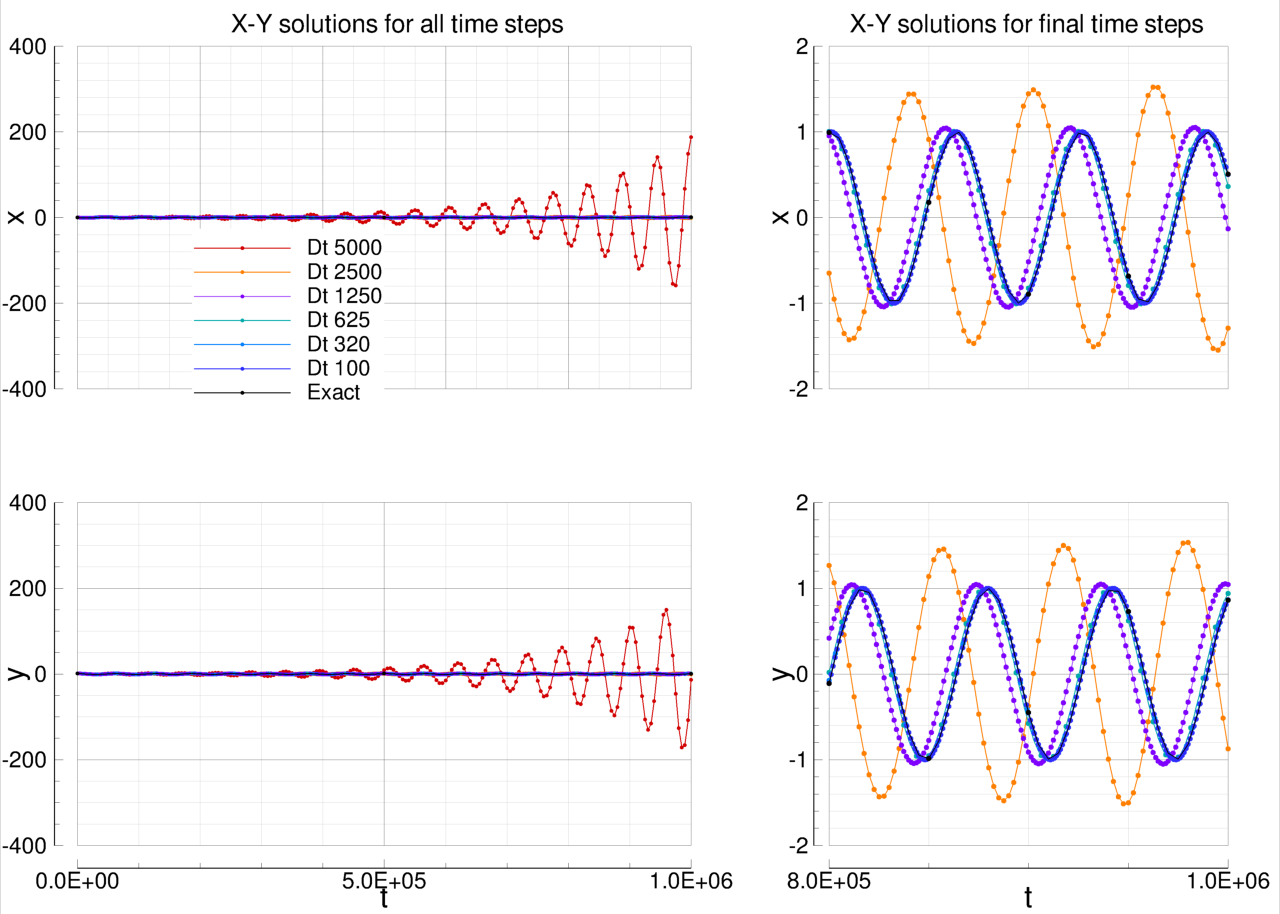
\includegraphics[width=1.00\textwidth]{errors-analysis/oscillation/errors_analysis-oscillation-adams-bashforth-2.png}
    \caption{Adams-Bashforth 2 steps solution}\label{fig:results-oscillation-adams-bashforth-2}
  \end{subfigure}\quad%
  \begin{subfigure}[b]{0.45\textwidth}
    \centering
    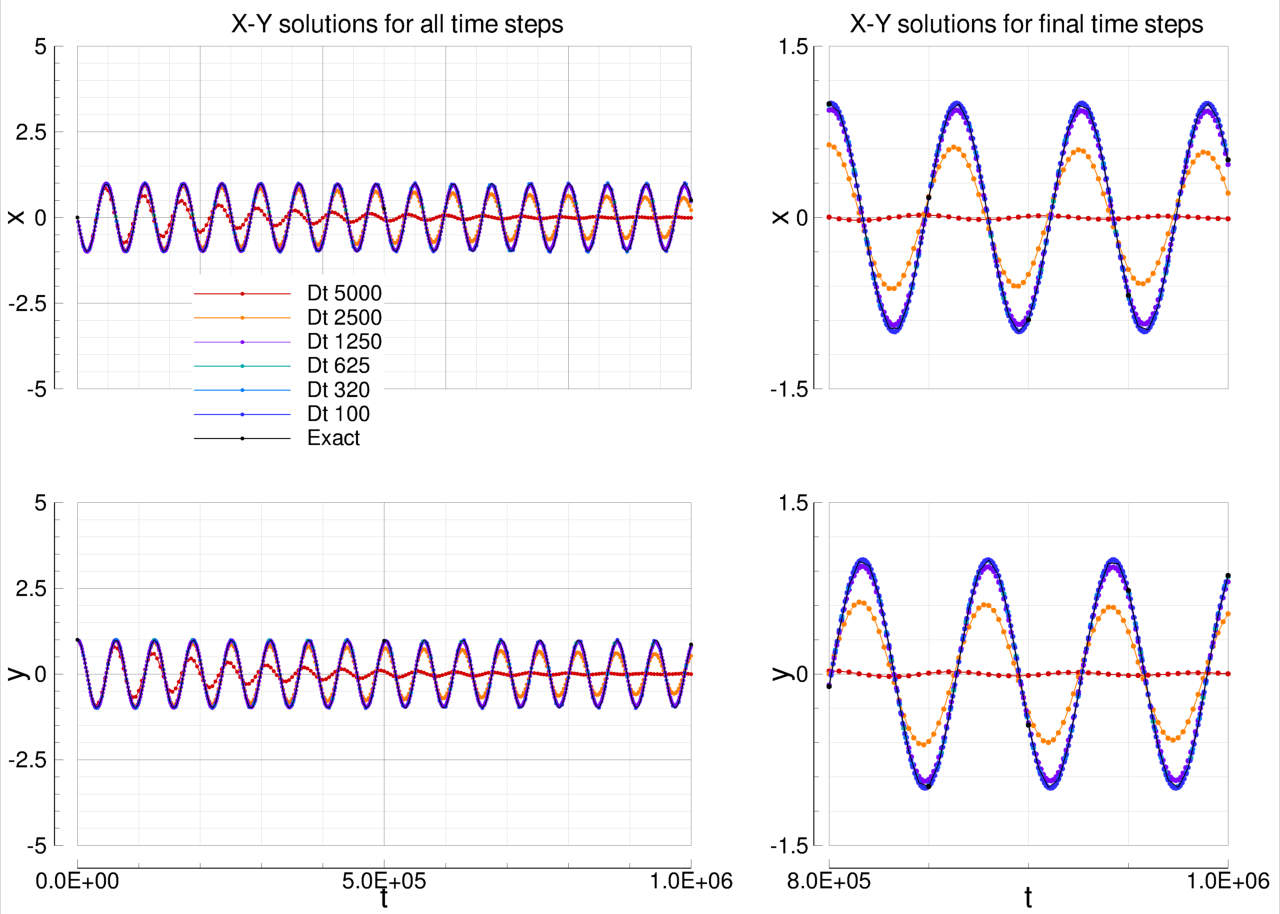
\includegraphics[width=1.00\textwidth]{errors-analysis/oscillation/errors_analysis-oscillation-adams-bashforth-3.png}
    \caption{Adams-Bashforth 3 steps solution}\label{fig:results-oscillation-adams-bashforth-3}
  \end{subfigure}\\
  \begin{subfigure}[b]{0.45\textwidth}
    \centering
    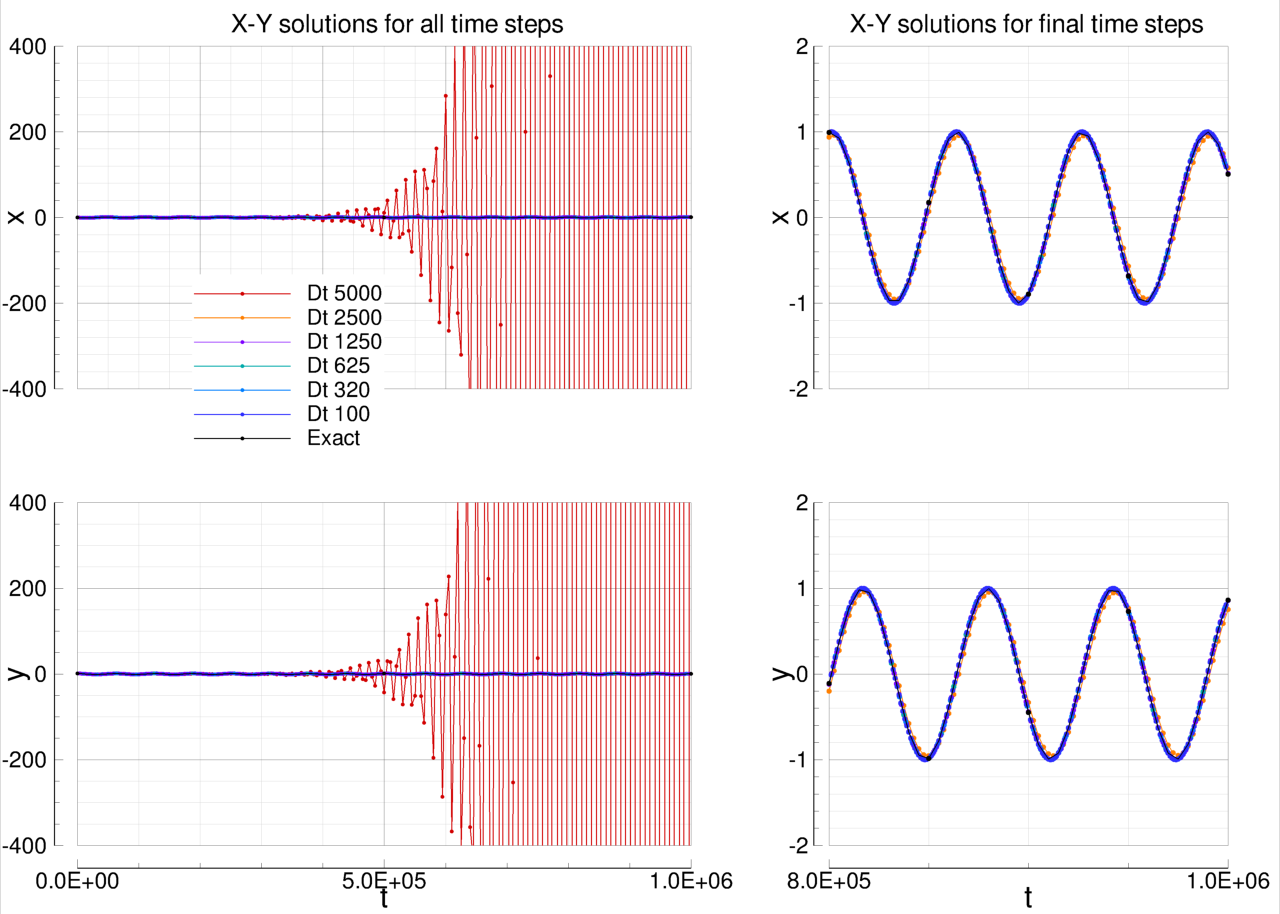
\includegraphics[width=1.00\textwidth]{errors-analysis/oscillation/errors_analysis-oscillation-adams-bashforth-4.png}
    \caption{Adams-Bashforth 4 steps solution}\label{fig:results-oscillation-adams-bashforth-4}
  \end{subfigure}
  \caption{Oscillation equations solutions computed by means of Adams-Bashforth solvers}\label{fig:results-oscillation-adams-bashforth}
\end{figure}

\paragraph{Leapfrog}

\begin{figure}[!ht]
  \centering
  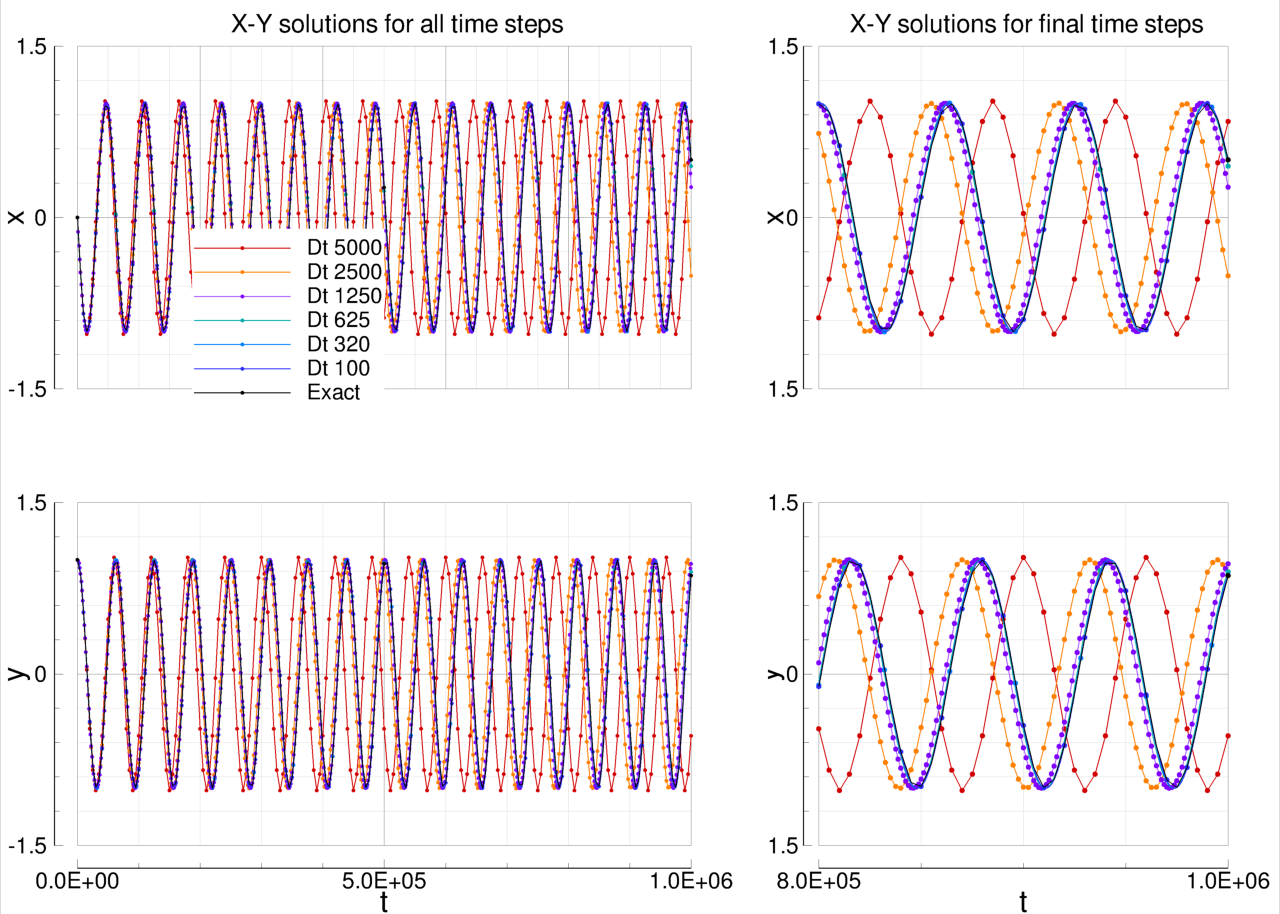
\includegraphics[width=0.70\textwidth]{errors-analysis/oscillation/errors_analysis-oscillation-leapfrog.png}
  \caption{Oscillation equations solutions computed by means of Leapfrog RAW-filtered solver}\label{fig:results-oscillation-leapfrog}
\end{figure}

\paragraph{Low Storage Runge-Kutta}

\begin{figure}[!ht]
  \centering
  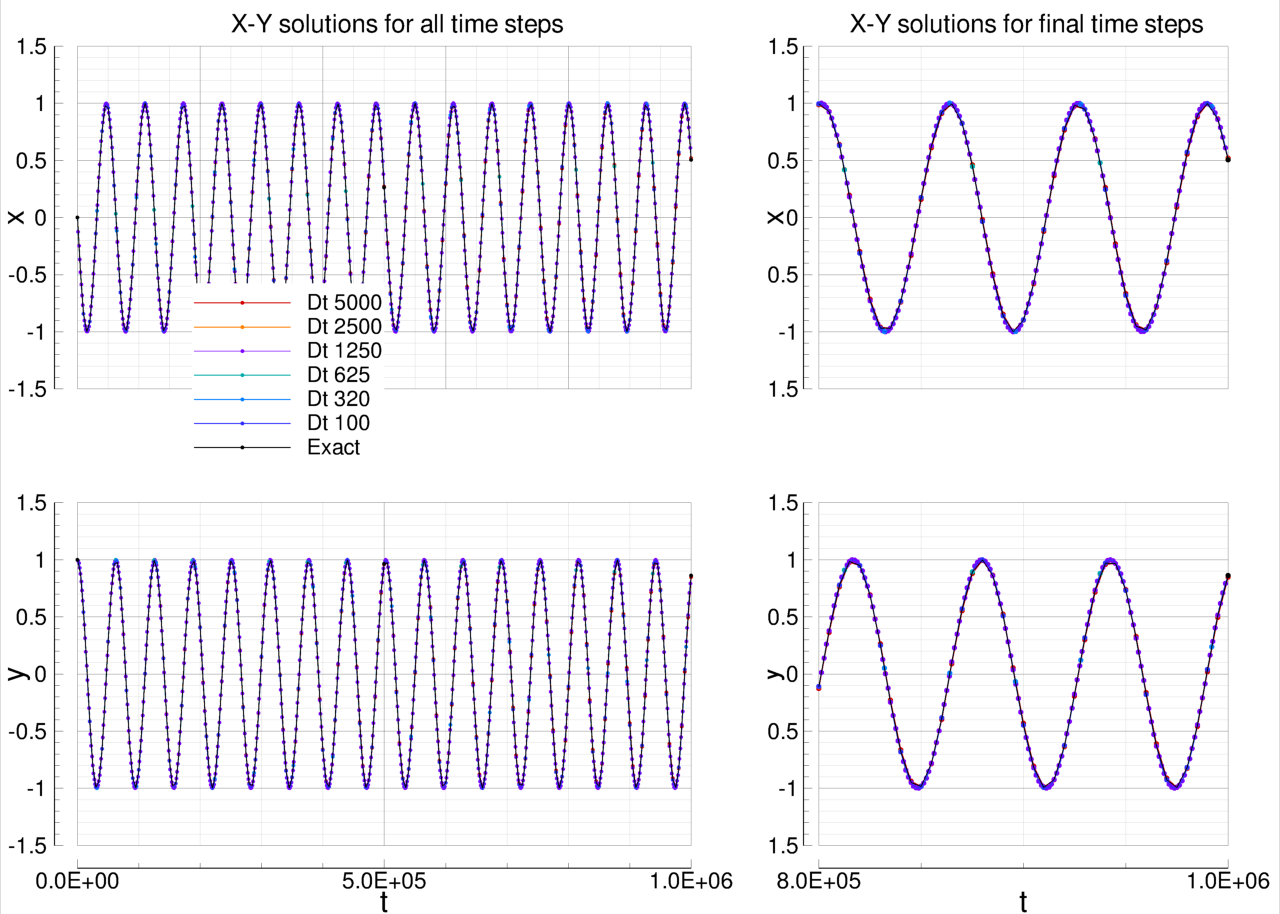
\includegraphics[width=0.70\textwidth]{errors-analysis/oscillation/errors_analysis-oscillation-ls-runge-kutta-5.png}
  \caption{Oscillation equations solutions computed by means of low storage Runge-Kutta 5 stages solver}\label{fig:results-oscillation-ls-runge-kutta-5}
\end{figure}

\paragraph{TVD/SSP Runge-Kutta}

\begin{figure}[!ht]
  \centering
  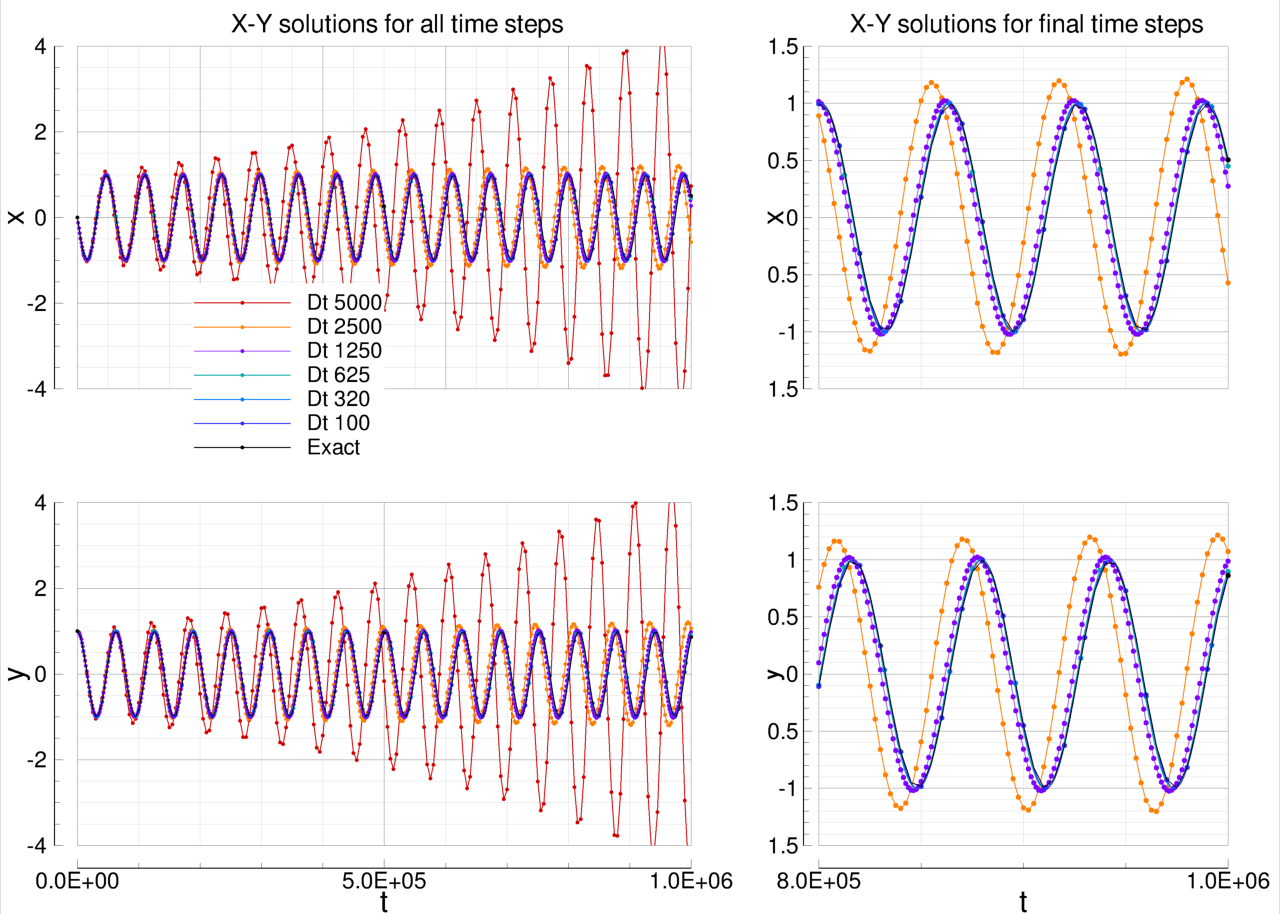
\includegraphics[width=0.70\textwidth]{errors-analysis/oscillation/errors_analysis-oscillation-tvd-runge-kutta-2.png}
  \caption{Oscillation equations solutions computed by means of TVD/SSP Runge-Kutta 2 stages solver}\label{fig:results-oscillation-tvd-runge-kutta-2}
\end{figure}

\begin{figure}[!ht]
  \centering
  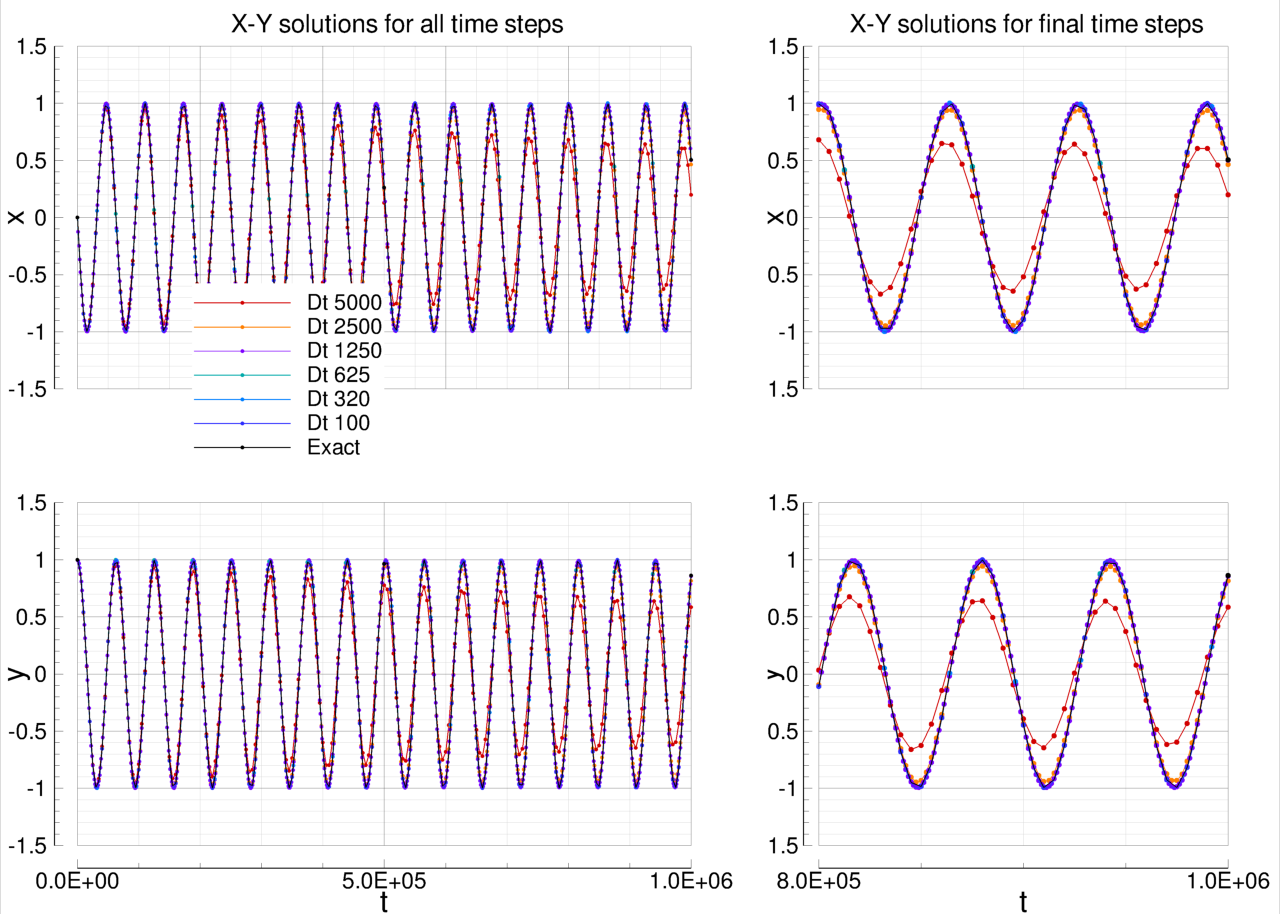
\includegraphics[width=0.70\textwidth]{errors-analysis/oscillation/errors_analysis-oscillation-tvd-runge-kutta-3.png}
  \caption{Oscillation equations solutions computed by means of TVD/SSP Runge-Kutta 3 stages solver}\label{fig:results-oscillation-tvd-runge-kutta-3}
\end{figure}

\begin{figure}[!ht]
  \centering
  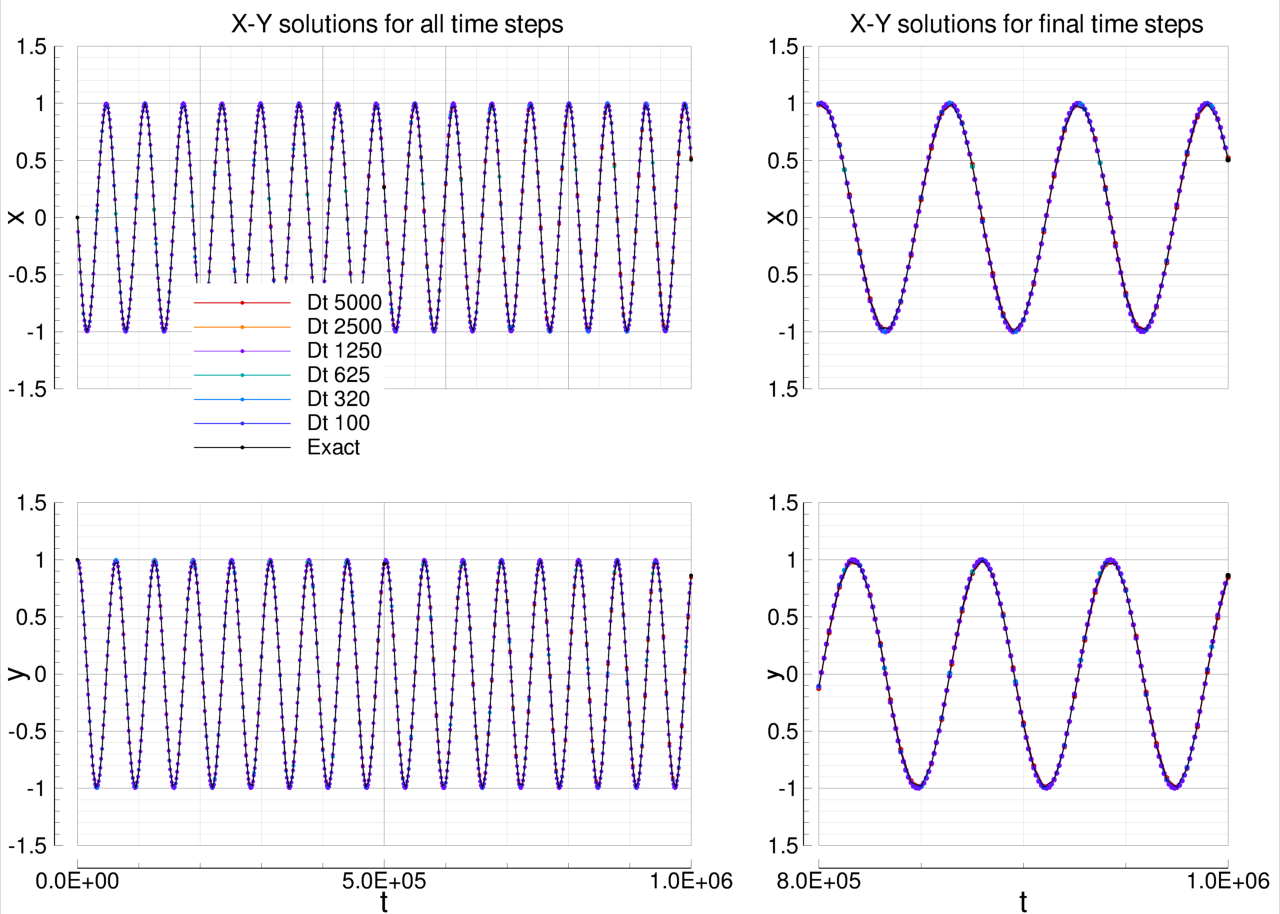
\includegraphics[width=0.70\textwidth]{errors-analysis/oscillation/errors_analysis-oscillation-tvd-runge-kutta-5.png}
  \caption{Oscillation equations solutions computed by means of TVD/SSP Runge-Kutta 5 stages solver}\label{fig:results-oscillation-tvd-runge-kutta-5}
\end{figure}

\clearpage

\section{Benchmarks on parallel frameworks}\label{sec:parallel}

{\color{red} To be written.}

\subsection{OpenMP benchmark}\label{subsec:openmp}

{\color{red} To be written.}

\subsection{MPI benchmark}\label{subsec:mpi}

{\color{red} To be written.}

\section{Concluding Remarks and Perspectives}\label{sec:conclusions}

{\color{red} To be written.}

\bibliographystyle{mycpc2}
\bibliography{Reference}

\end{document}
